%%=============================================================================
%% Methodologie
%%=============================================================================

\chapter{\IfLanguageName{dutch}{Methodologie}{Methodology}}%
\label{ch:methodologie}

%% TODO: In dit hoofstuk geef je een korte toelichting over hoe je te werk bent
%% gegaan. Verdeel je onderzoek in grote fasen, en licht in elke fase toe wat
%% de doelstelling was, welke deliverables daar uit gekomen zijn, en welke
%% onderzoeksmethoden je daarbij toegepast hebt. Verantwoord waarom je
%% op deze manier te werk gegaan bent.
%% 
%% Voorbeelden van zulke fasen zijn: literatuurstudie, opstellen van een
%% requirements-analyse, opstellen long-list (bij vergelijkende studie),
%% selectie van geschikte tools (bij vergelijkende studie, "short-list"),
%% opzetten testopstelling/PoC, uitvoeren testen en verzamelen
%% van resultaten, analyse van resultaten, ...
%%
%% !!!!! LET OP !!!!!
%%
%% Het is uitdrukkelijk NIET de bedoeling dat je het grootste deel van de corpus
%% van je bachelorproef in dit hoofstuk verwerkt! Dit hoofdstuk is eerder een
%% kort overzicht van je plan van aanpak.
%%
%% Maak voor elke fase (behalve het literatuuronderzoek) een NIEUW HOOFDSTUK aan
%% en geef het een gepaste titel.

\section{Literatuuronderzoek}

In het literatuuronderzoek zijn we in detail op zoek gegaan naar de mogelijkheden die er zijn om ETL's en ELT's te gaan implementeren. Hierbij houden we rekening dat Net IT met Microsoft producten werkt waardoor er vooral naar Azure gekeken wordt. Er is dus ook verder in detail gegaan op deze Azure producten doordat deze meer aan bod komen in de bachelorproef.

\section{Long list}

Hier alle mogelijkheden voor het implementeren van ETL's/ELT's opnoemen? Dit kan een lange lijst worden met mogelijkheden die niet relevant zijn voor Net IT aangezien er van Azure gebruik gemaakt wordt. Is dit een stap die dus overgeslaan kan worden?

\section{Short list}

Op basis van de long list houden we twee mogelijkheden over voor het implementeren van ELT's en ETL's. Dit zijn Azure Data Factory en Azure Databricks. Er is gekozen voor deze twee technologieën doordat deze beide van Azure zijn. 

\section{Vergelijkingscriteria}

\subsection{Kostprijs}

\subsection{Performantie}

\subsection{Mogelijkheid tot debuggen}

\subsection{Verschil in implementatietijd}

\subsection{Moeilijkheidsgraad in opzet}

\subsection{Mogelijkheden van de tool}

\subsection{Onderhoudbaarheid}

\subsection{Testbaarheid}

\section{Proof-of-concepts}


Binnen Net IT wordt data van Microsoft 365 Customer Engagement geëxporteerd naar naar CSV bestanden en in Azure Data Lake geplaatst. Deze bestanden moeten minstens één keer per dag opgesplitst worden per groep per jaar en zullen moeten doorgestuurd worden naar de klant. Hiervoor moet er dus een ETL of ELT geïmplementeerd worden. Doordat er onderzocht zal worden naar wat de beste mogelijkheid is voor het implementeren van deze ETL of ELT zal er dus een proof-of-concept uitgewerkt worden voor zowel Azure Data Factory en Azure Databricks. Voor het implementeren van deze proof-of-concepts zal er een pipeline gemaakt worden die ook bij de klant gebruikt wordt. Belangrijk hierbij is dat er voor deze bachelorproef gebruik gemaakt zal worden van dummy data.
    

De tabellen uit data lake die gebruikt worden zijn `new\_syndicalpremiumrequest`, `new\_person`, `new\_bankaccount`, `new\_year`, `new\_membership`, `new\_group` en `new\_organizationyear`. Voor zowel Data Factory als Databricks zal er eerst gekeken worden naar hoe deze opgezet kunnen worden. Vervolgens zal er gekeken worden naar hoe er samen gewerkt kan worden en hoe source control geïmplementeerd kan worden. Daarnaast zal er gekeken worden hoe men data kan ophalen uit data lake met behulp van het Common Data Model en zullen de belangrijkste transformaties overlopen worden. Op deze manier kan Data Factory en Databricks makkelijk vergeleken worden.
    

Er zal steeds gewerkt worden vanuit de tabel `new\_syndicalpremiumrequest`. Dit zijn de premies die geëxporteerd worden vanuit Microsoft 365 Customer Engagement. Deze premies zullen dus opgesplitst worden per groep, per jaar. Voor de pipelines die nu geïmplementeerd worden, worden de premies naar één CSV bestand geëxporteerd. Dit zodat het geëxporteerde CSV bestand van Data Factory dan makkelijk vergeleken kan worden met het geëxporteerde CSV bestand van Databricks.

\subsection{Azure Data Factory (ADF)}

\subsubsection{Opzet van resources}

\begin{center}
    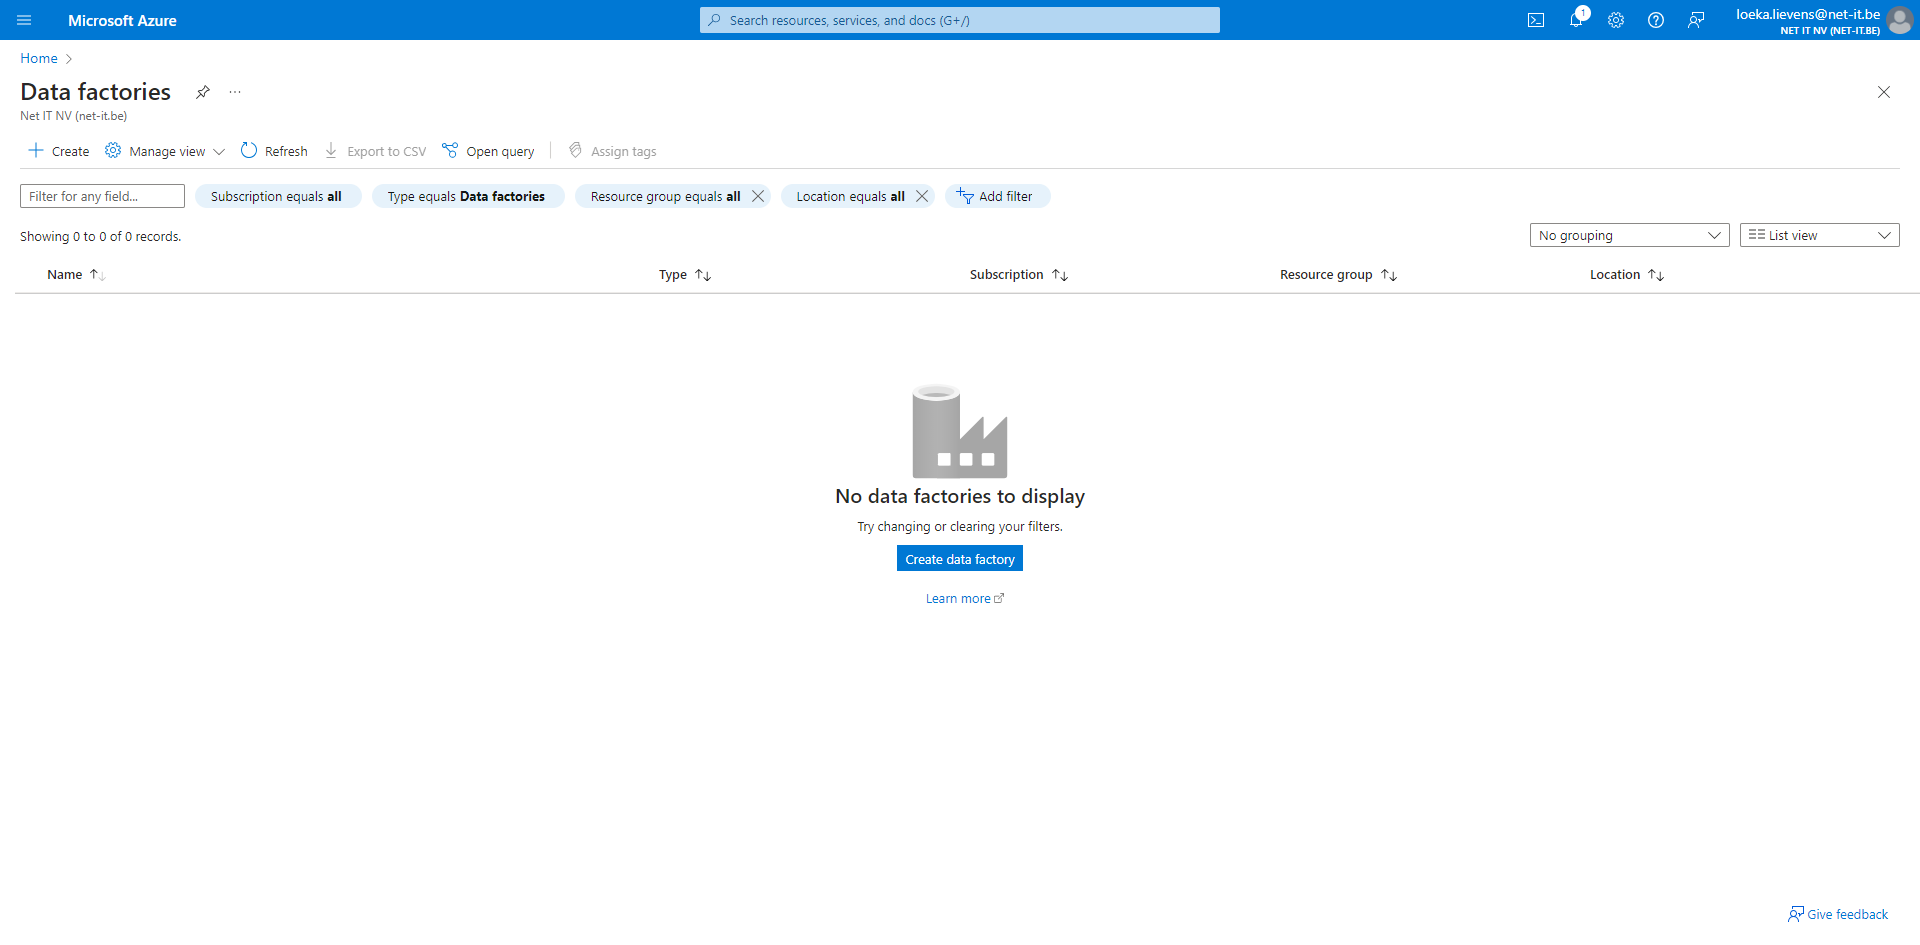
\includegraphics[width=0.6\textwidth]{./graphics/adf/initial.png}
    \footnote{Aanmaken van Azure Data Factory}
\end{center}

Door in Microsoft Azure naar Data Factories te navigeren kunnen we een nieuwe data factory gaan aanmaken.

\begin{center}
    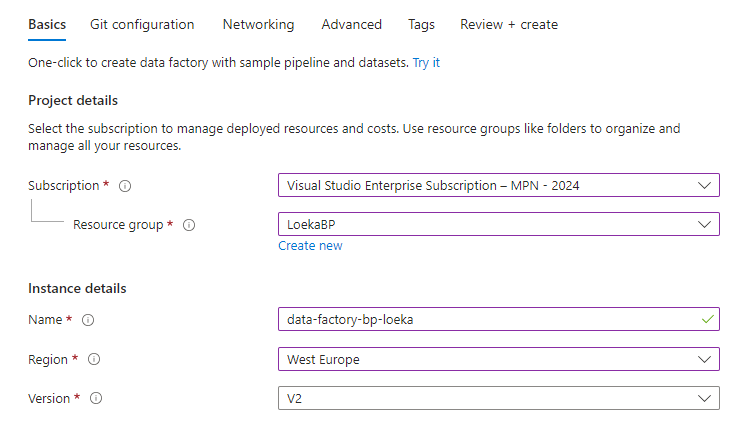
\includegraphics[width=0.6\textwidth]{./graphics/adf/initial_create.png}
    \footnote{Configuratie van Azure Data Factory}
\end{center}

% Resource group en subscription in literatuurstudie
Bij het aanmaken van een data factory moet er een subscription en resource group gekozen worden. Er kan een nieuwe resource group aangemaakt worden of een reeds bestaande gekozen worden. Daarnaast moet er een naam, gewenste regio en versie voor Data Factory gekozen worden. Git configuratie zal later aan bod komen. Data Factory kan nu aangemaakt worden.

\begin{center}
    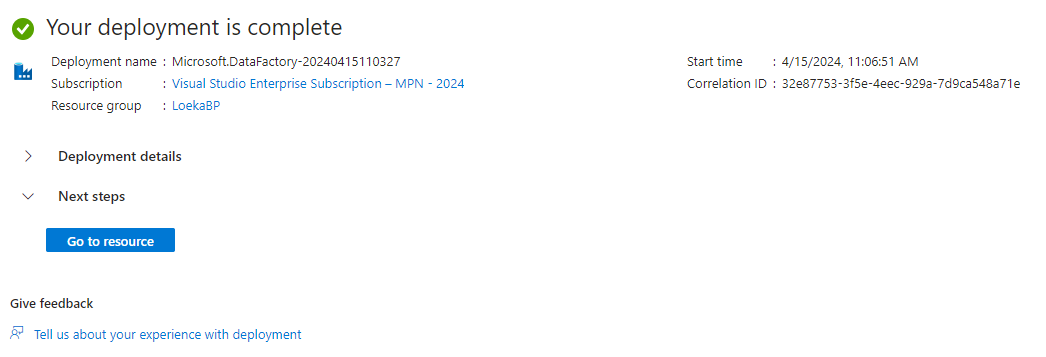
\includegraphics[width=0.6\textwidth]{./graphics/adf/deployment_complete_specific.png}
    \footnote{Deployment complete van Azure Data Factory}
\end{center}

Wanneer de resource is aangemaakt kan Azure Data Factory opgestart worden.

\subsubsection{Collaboration en source control}

Binnen Azure Data Factory kan er op 2 manieren samen gewerkt worden. 

\begin{center}
    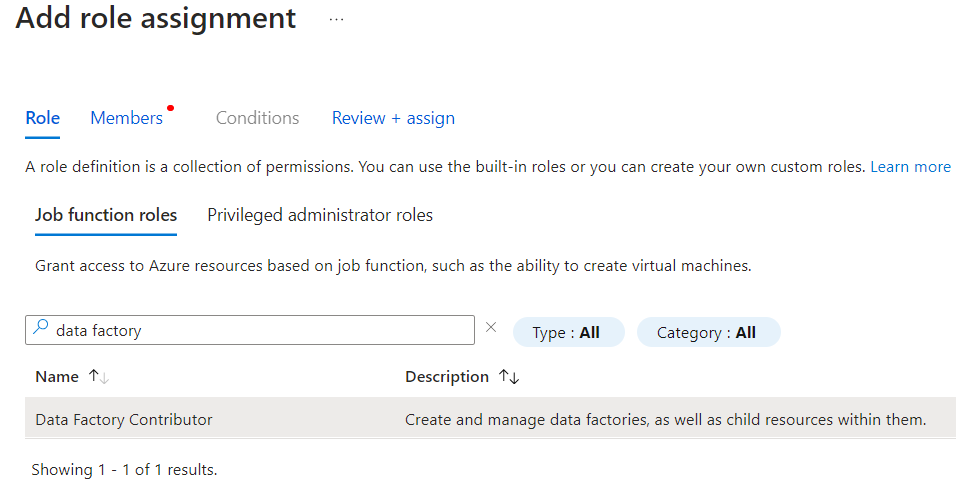
\includegraphics[width=0.6\textwidth]{./graphics/adf/adf_contributor.png}
    \footnote{Toewijzen van Data Factory Contributor Role}
\end{center}

Door de bij de resource group van de data factory de Data Factory Contributor role toe te wijzen kan men toegang geven tot volgende zaken:
\begin{itemize}
    \item Het aanmaken, wijzigen en verwijderen van data factories en child resources
    \item Deployment van Resource Manager templates
    \item Het managen van App Insight alerts voor Data Factory
    \item Het aanmaken van support tickets
\end{itemize}

Daarnaast kan er ook samen gewerkt worden via source control. Azure Data Factory laat het toe om een Git repository te configureren via Azure Repos of GitHub. 

\begin{center}
    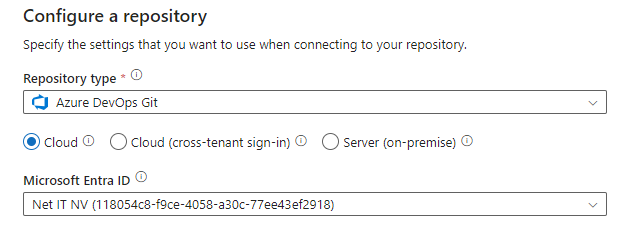
\includegraphics[width=0.6\textwidth]{./graphics/adf/setup_repository_2_specific.png}
    \footnote{Configuratie van Git in Azure Data Factory}
\end{center}

We kiezen voor Azure DevOps doordat er binnen Net IT hiermee gewerkt wordt.

\begin{center}
    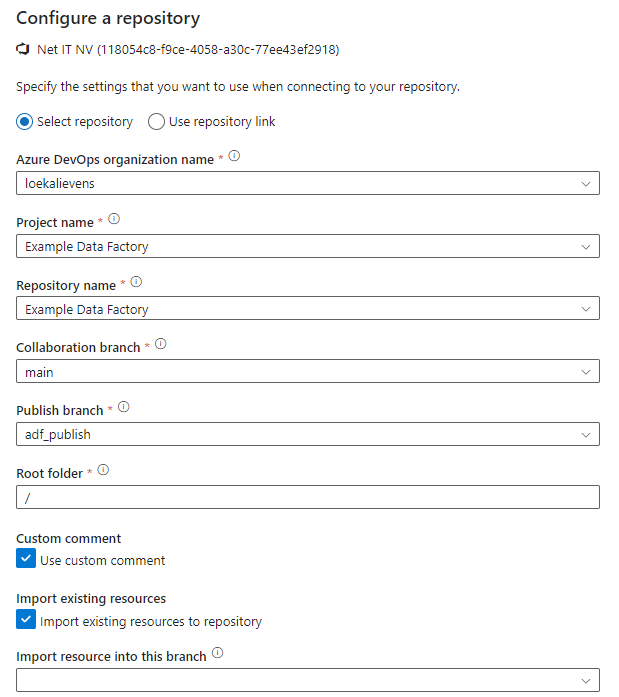
\includegraphics[width=0.6\textwidth]{./graphics/adf/setup_repository_3_specific.png}
    \footnote{Configuratie van Azure DevOps in Azure Data Factory}
\end{center}

De collaboration branch is de enigste branch waarbij de publish knop zichtbaar zal zijn. Door te werken met feature branches en hiermee pull requests te maken op de collaboration branch kan er dus samen gewerkt worden. De publish branch is de branch waar alle ARM templates van de gepubliceerde factory opgeslaan wordt.

\subsubsection{Ophalen van data uit Azure Data Lake}

Het ophalen van data uit Data Lake in Data Flow zal steeds op dezelfde manier gebeuren. 

\begin{center}
    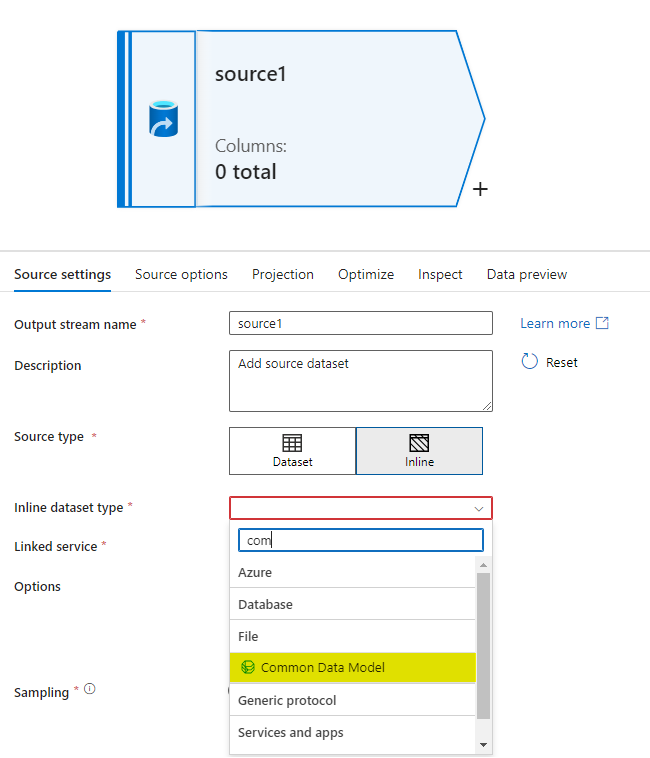
\includegraphics[width=0.6\textwidth]{./graphics/adf/source_table_1_specific.png}
    \footnote{Configuratie van source transformation}
\end{center}

Als source type zal er steeds gekozen worden voor inline. Dit doordat we slechts werken met één enkele dataflow en geen gedeelde datasets nodig hebben. Als inline data set type kiezen we voor Common Data Model.

\begin{center}%
    \centering
    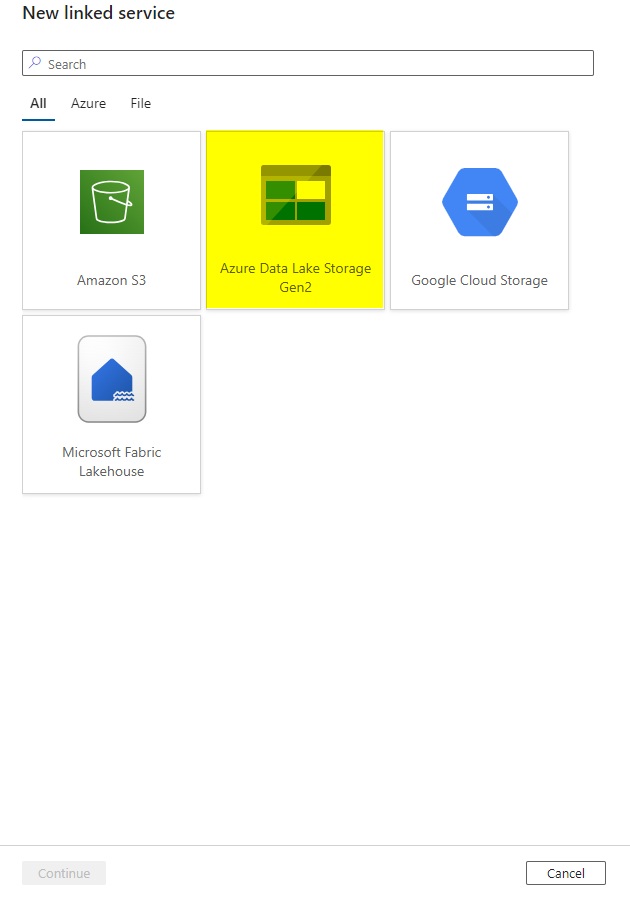
\includegraphics[width=0.4\textwidth]{./graphics/adf/source_table_2_specific}
    \hspace{0.1\textwidth}
    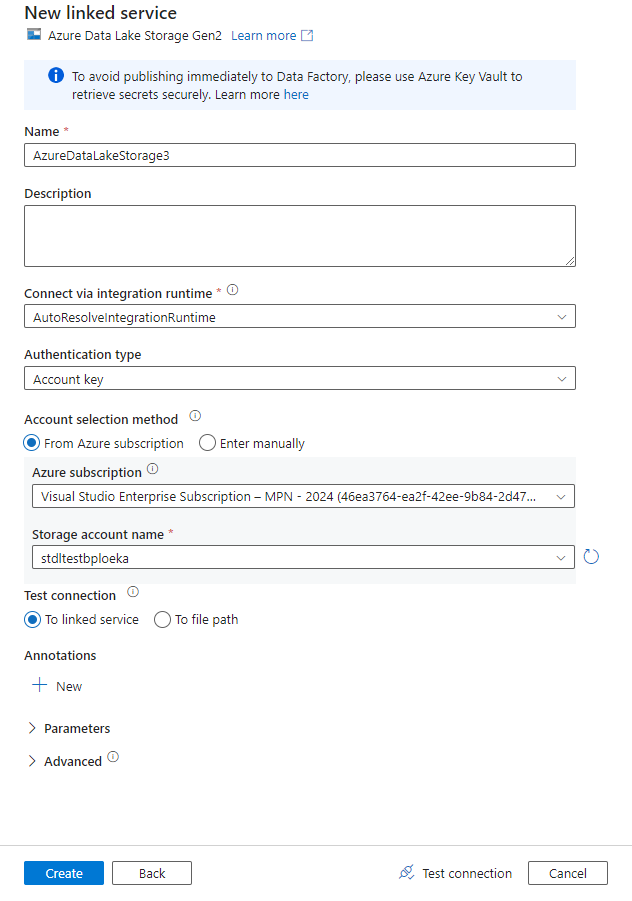
\includegraphics[width=0.4\textwidth]{./graphics/adf/source_table_3_specific}
    \footnote{Configuratie van linked service}
\end{center}

Er zal éénmalig een Linked Service aangemaakt moeten worden. Hierbij kiezen we voor Azure Data Lake Storage Gen2. We kunnen makkelijk gaan koppelen met de juiste data lake door een Azure Subscription en Storage account name aan te duiden. Door op `Test connection` te klikken kunnen we kijken of de connectie met data lake is gelukt. Door op `Create` te klikken hebben we nu een Linked Service die steeds bij elke Source gebruikt kan worden.

\textbf{Let op:} Doordat Git geen secrets opslaat is het aanbevolen om gebruik te maken van Azure Key Vault voor het opslaan van connection strings of passwords.

\begin{center}
    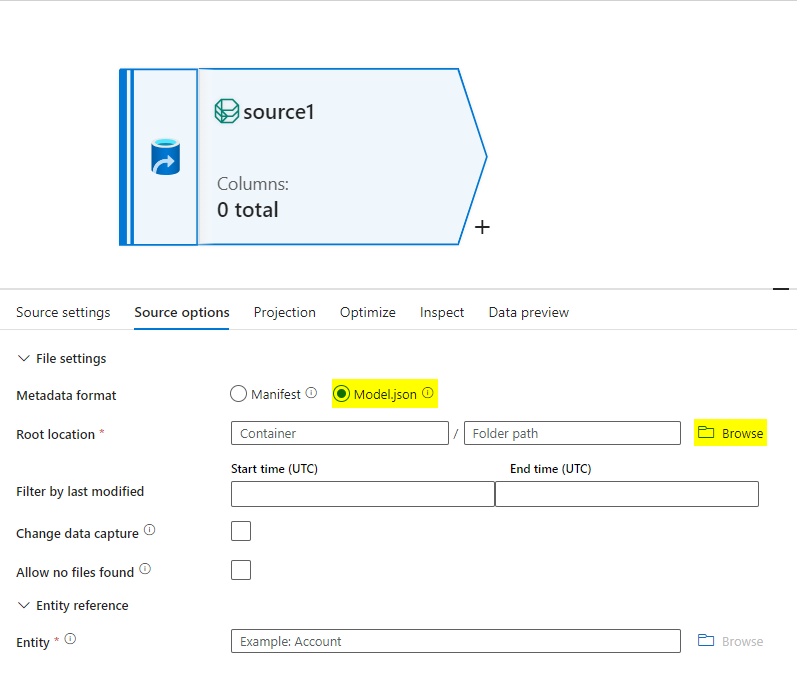
\includegraphics[width=0.6\textwidth]{./graphics/adf/source_table_4_specific.png}
    \footnote{Configuratie van source options}
\end{center}

Door naar `Source options` te gaan kunnen we `Model.json` gaan aanduiden. Door op `Browse` te klikken kunnen we aanduiden waar het Model.json bestand te vinden is in data lake.

\begin{center}
    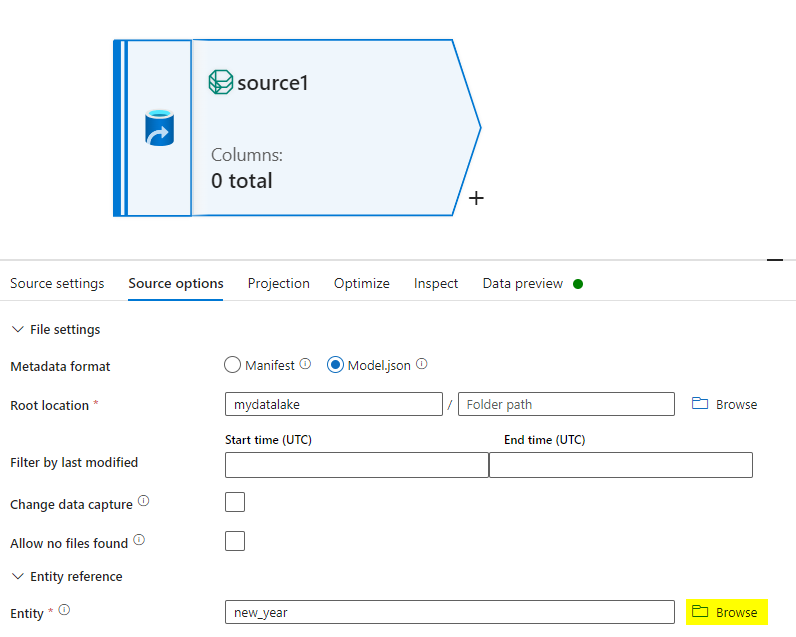
\includegraphics[width=0.6\textwidth]{./graphics/adf/source_table_5_specific.png}
    \footnote{Configuratie van source options}
\end{center}

Naast `Entity` kunnen we nu op `Browse` klikken om de gewenste entity te gaan importeren. Let op: hier voor zal Data flow debug aan moeten staan.

\begin{center}
    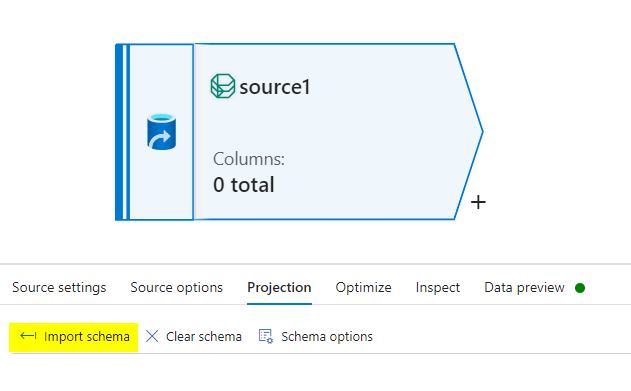
\includegraphics[width=0.6\textwidth]{./graphics/adf/source_table_6_specific.png}
    \footnote{Configuratie van projection}
\end{center}

Door naar `Projection` te gaan kunnen we nu op `Import schema` klikken.

\begin{center}
    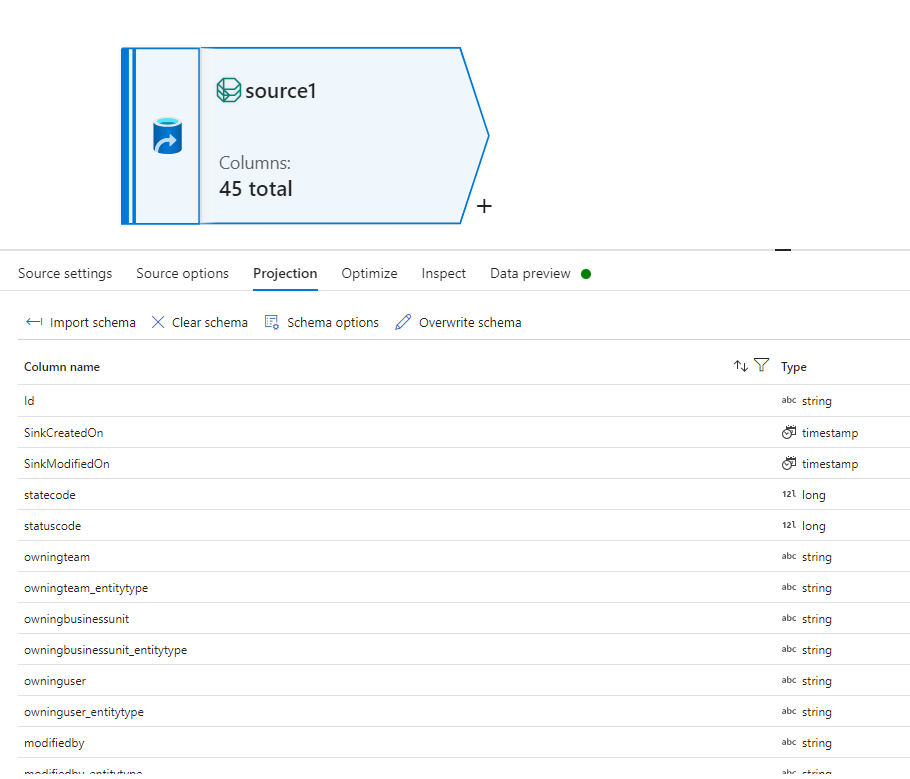
\includegraphics[width=0.6\textwidth]{./graphics/adf/source_table_7_specific.png}
    \footnote{Configuratie van projection}
\end{center}

De foto hierboven toont een voorbeeld van een geïmporteerd schema.

\begin{center}
    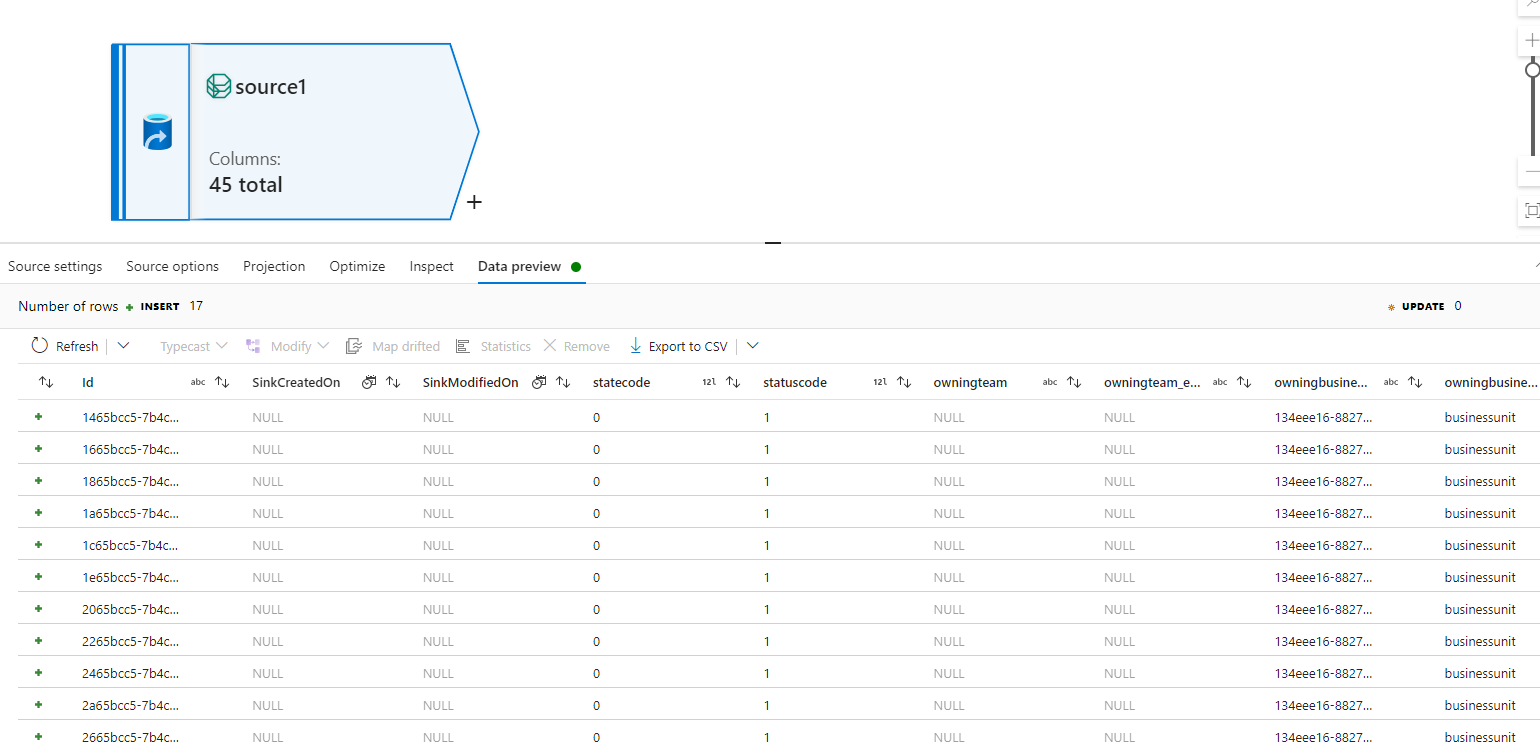
\includegraphics[width=0.6\textwidth]{./graphics/adf/source_table_8_specific.png}
    \footnote{Data preview}
\end{center}

Wanneer we naar `Data preview` gaan kunnen we een preview zien van de data uit de gekozen tabel.

\subsubsection{Belangrijkste transformaties}

Determinatie van welke groepen de premie in hun bestand krijgen

\begin{center}
    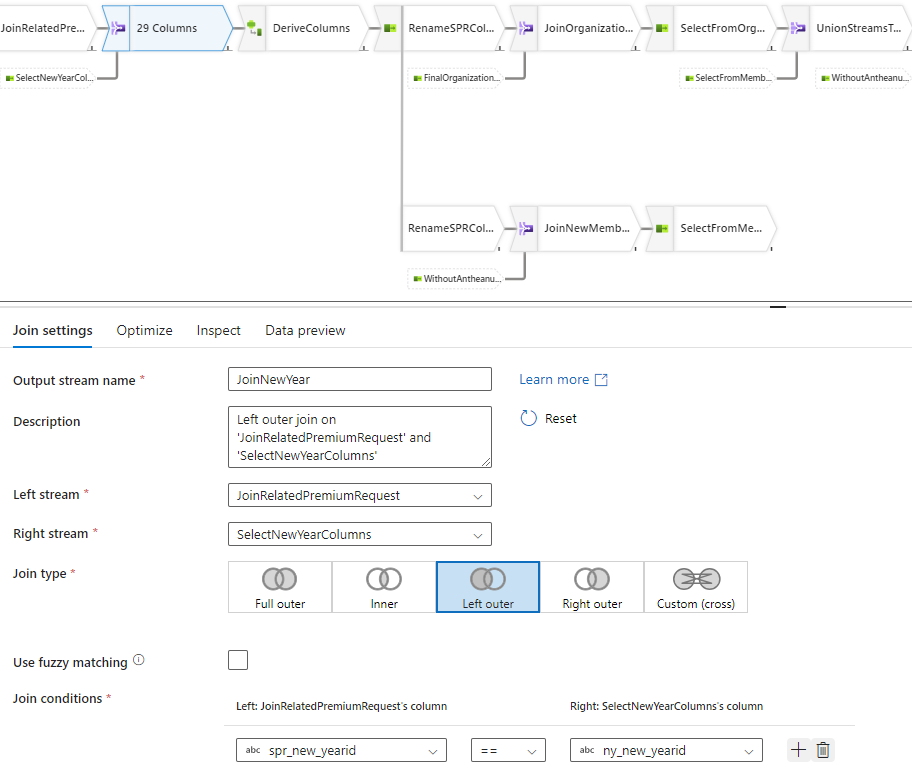
\includegraphics[width=0.6\textwidth]{./graphics/adf/bepalen_groep_1.png}
    \footnote{Join van de tabel `new\_year` op de tabel `new\_syndicalpremiumrequest`}
\end{center}

De tabel `new\_syndicalpremiumrequest` heeft een kolom `spr\_new\_yearid`. Om te gaan bepalen wat het referentiejaar van deze premie is zal dus de tabel `new\_year` op de tabel `new\_syndicalpremiumrequest` gejoind moeten worden aan de hand van dit id.


\begin{center}
    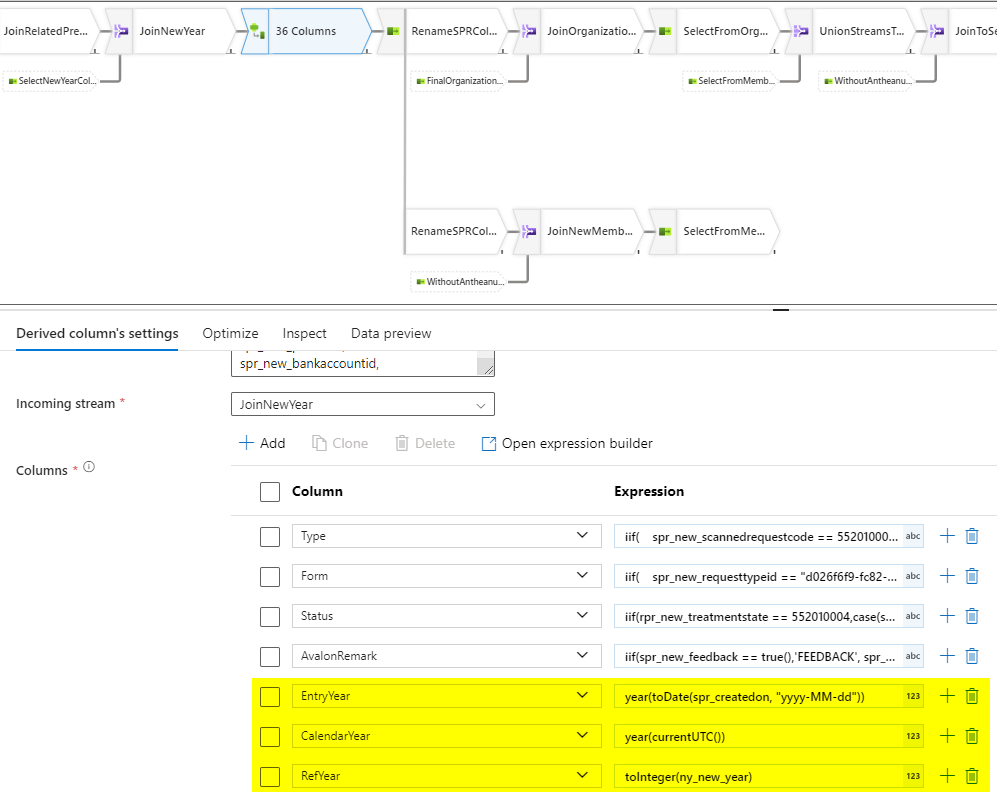
\includegraphics[width=0.6\textwidth]{./graphics/adf/bepalen_groep_2.png}
    \footnote{Derive EntryYear, CalendarYear en RefYear op de tabel `new\_syndicalpremiumrequest`}
\end{center}

Voor het bepalen van de groepen moeten hebben we 3 nieuwe kolommen nodig. Als eerste hebben we het EntryYear nodig, dit is het jaartal van `spr\_createdon`, de datum wanneer de record is aangemaakt. Daarnaast hebben we CalendarYear nodig, dit is het jaartal van de huidige datum. En ten slotte hebben we RefYear nodig, dit is het jaartal van de tabel `new\_year` die net gejoind is geweest.

\begin{center}
    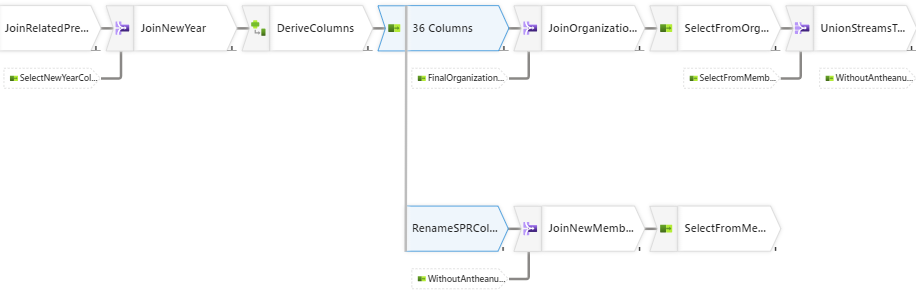
\includegraphics[width=0.6\textwidth]{./graphics/adf/bepalen_groep_3.png}
    \footnote{Hernoemen van `new\_syndicalpremiumrequest` kolommen en splitsing in twee apparte branches}
\end{center}

Vervolgens worden bepaalde kolommen van naam hernoemt. Welke kolommen dit zijn is onbelangrijk voor deze transformatie. Wat wel belangrijk is dat de pipeline zich nu opsplitst in twee apparte branches. Dit doordat er 2 inner joins zullen gebeuren.

\begin{center}
    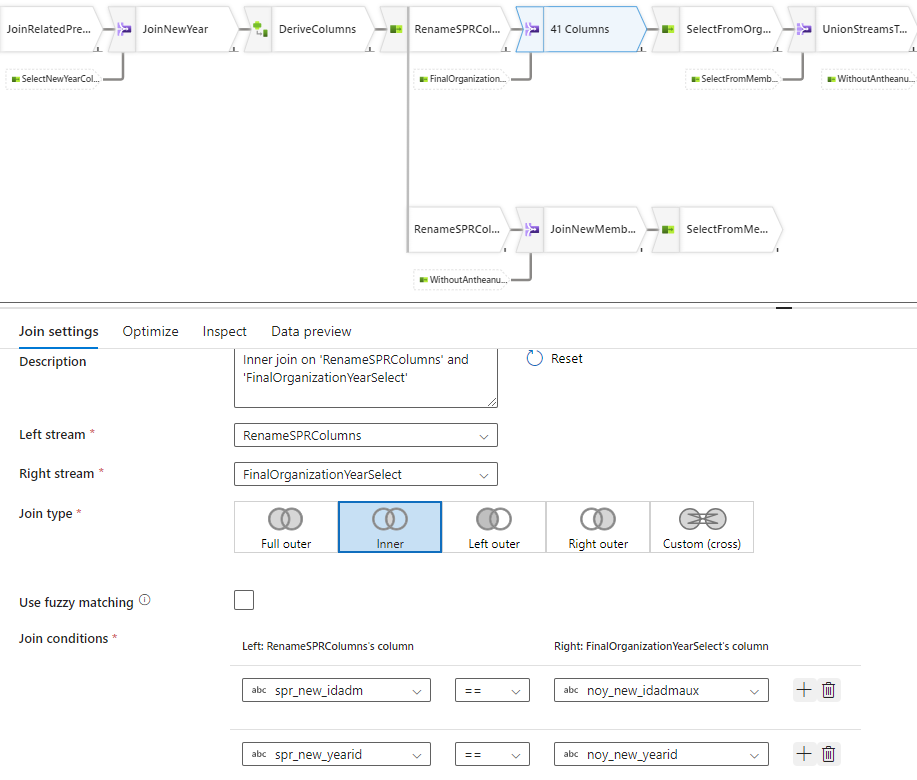
\includegraphics[width=0.6\textwidth]{./graphics/adf/bepalen_groep_4.png}
    \footnote{Inner join van `new\_organizationyear` op de tabel `new\_syndicalpremiumrequest`}
\end{center}

Er gebeurt nu een inner join van de tabel `new\_organizationyear` op de tabel `new\_syndicalpremiumrequest`. Hierbij wordt er aan de hand van IDADM en het id van het referentiejaar gejoind.

\begin{center}
    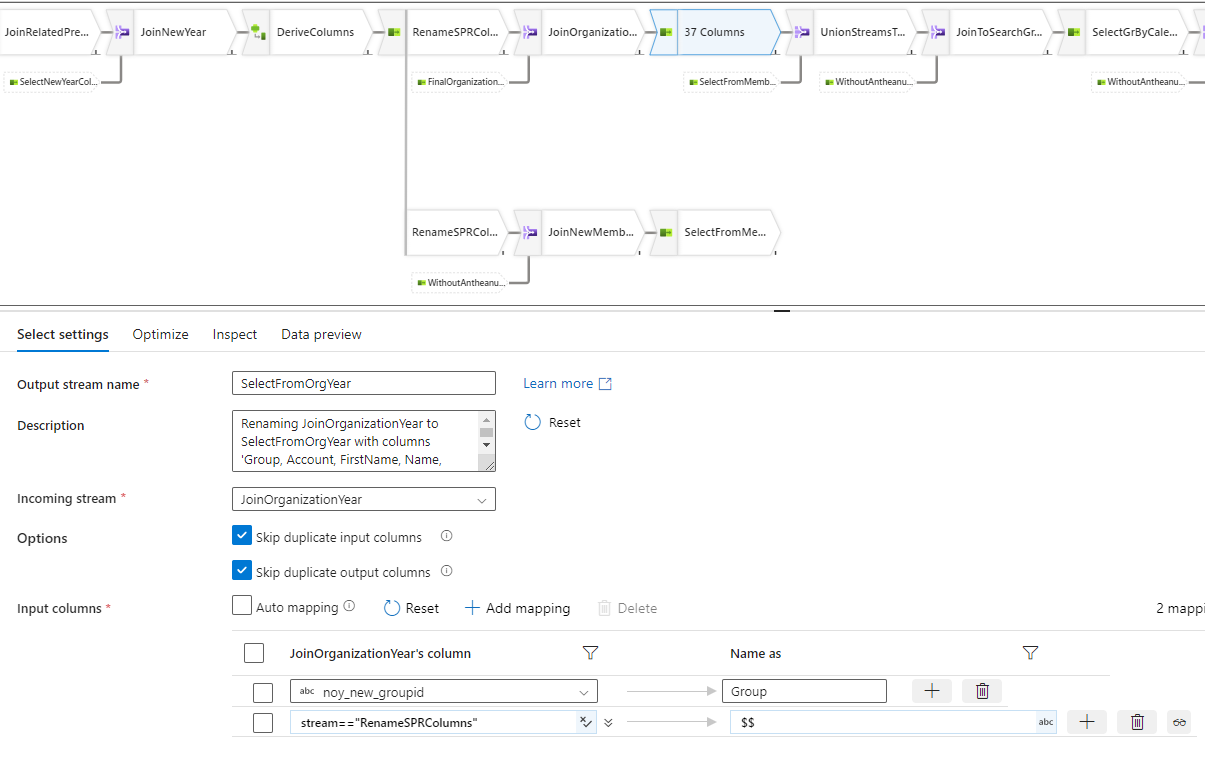
\includegraphics[width=0.6\textwidth]{./graphics/adf/bepalen_groep_5.png}
    \footnote{Selecteren en hernoemen van kolommen op de tabel `new\_syndicalpremiumrequest`}
\end{center}

Vervolgens worden alle kolommen die er voor de join waren geselecteerd. Daarnaast wordt er één kolom `noy\_new\_groupid` geselecteerd en hernoemd naar `Group`.

\begin{center}
    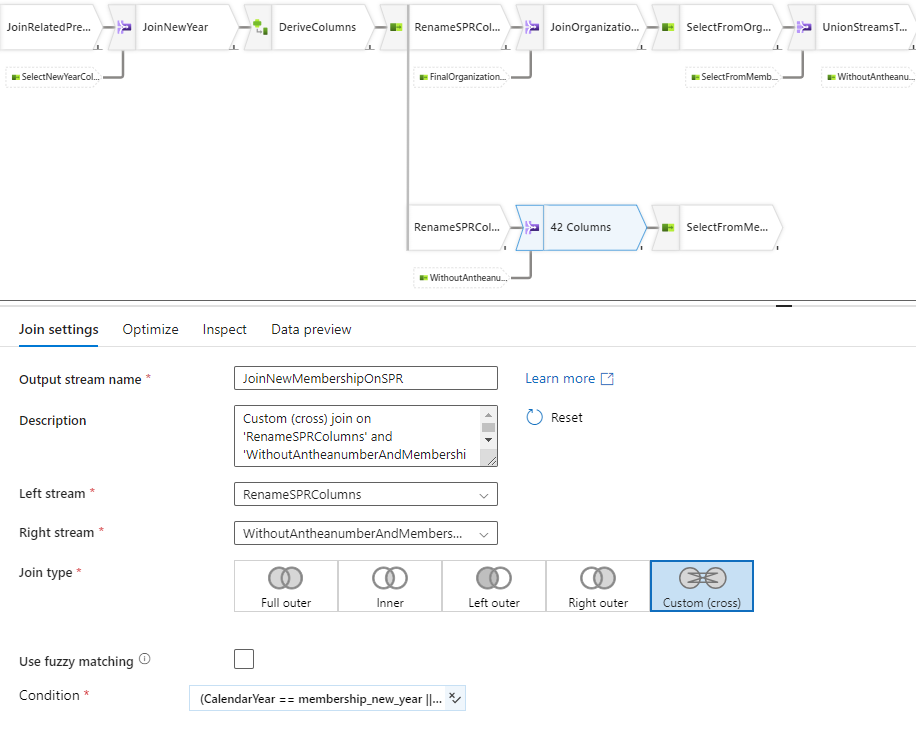
\includegraphics[width=0.6\textwidth]{./graphics/adf/bepalen_groep_6.png}
    \footnote{Custom (cross) join van `new\_membership` op de tabel `new\_syndicalpremiumrequest`}
\end{center}

Bij de tweede branch wordt de tabel `new\_membership` gejoind op de tabel `new\_syndicalpremiumrequest`. Er wordt gebruik gemaakt van een custom (cross) join doordat er OR condities worden gebruikt. 

\begin{center}
    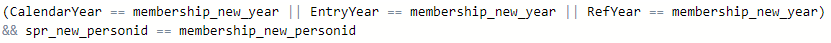
\includegraphics[width=0.6\textwidth]{./graphics/adf/bepalen_groep_7.png}
    \footnote{Conditie van de custom (cross) join van `new\_membership` op de tabel `new\_syndicalpremiumrequest`}
\end{center}

In de conditie van de custom (cross) join wordt er vergeleken of CalendarYear, EntryYear of RefYear overeenkomt met het jaartal van de membership. Daarnaast wordt er ook gekeken of personid overeen komt.

\begin{center}
    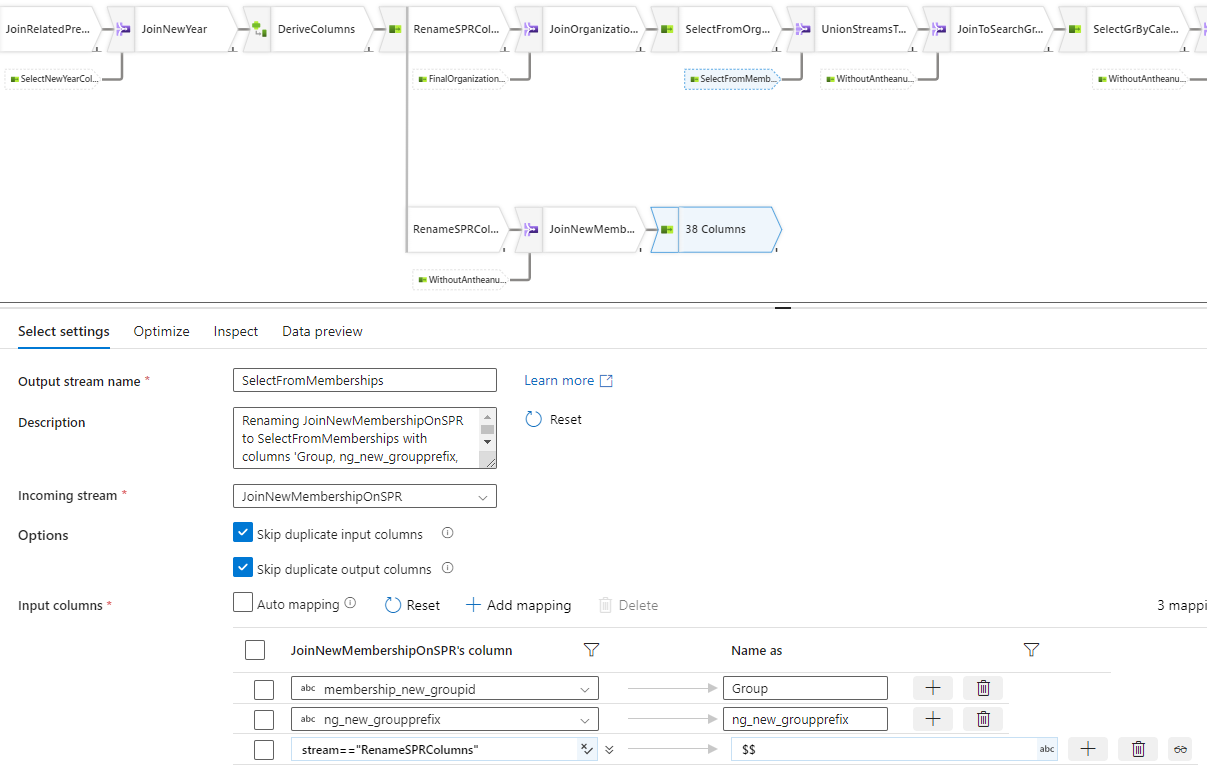
\includegraphics[width=0.6\textwidth]{./graphics/adf/bepalen_groep_8.png}
    \footnote{Selecteren en hernoemen van kolommen op de tabel `new\_syndicalpremiumrequest`}
\end{center}

Ook na deze join worden alle kolommen die er voor de join waren geselecteerd. Daarnaast wordt er 1 kolom `membership\_new\_groupid` geselecteerd en hernoemd naar `Group`. Ten slotte wordt de kolom `ng\_new\_groupprefix` geselecteerd maar dit heeft te maken met een andere transformatie.

\begin{center}
    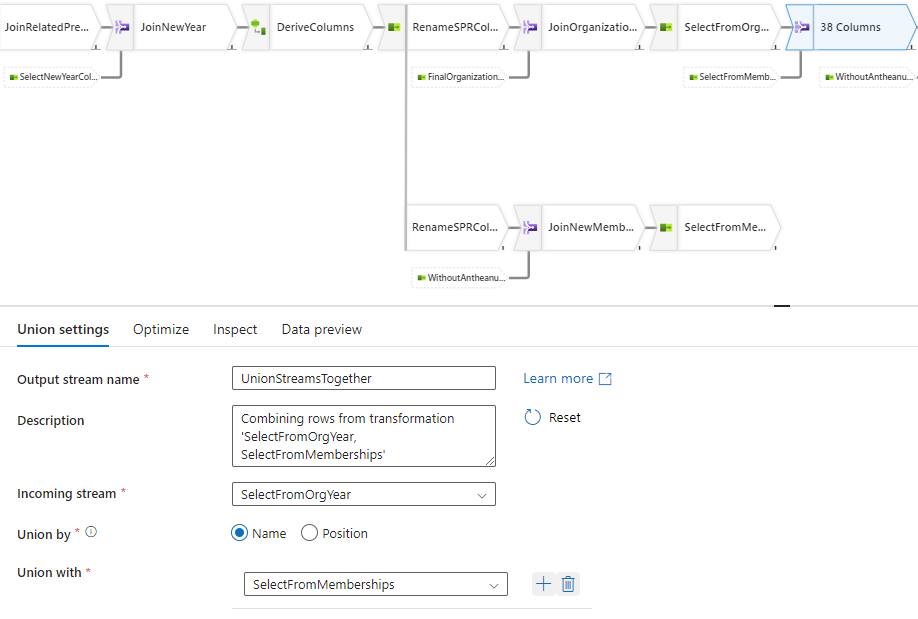
\includegraphics[width=0.6\textwidth]{./graphics/adf/bepalen_groep_9.png}
    \footnote{Union van twee branches}
\end{center}

Beide branches hebben nu dezelfde kolommen met een extra kolom `Group`. Daarnaast heeft de onderste branch nog één extra kolom `ng\_new\_groupprefix`. De beide branches worden nu samen gevoegd met behulp van een union. De bovenste branch die de kolom `ng\_new\_groupprefix` niet heeft zal voor deze kolom de waarde `NULL` krijgen in de records komende van deze branch. 

% TODO group by uitleggen

\subsection{Azure Databricks}

\subsubsection{Opzet van resources}

\begin{center}
    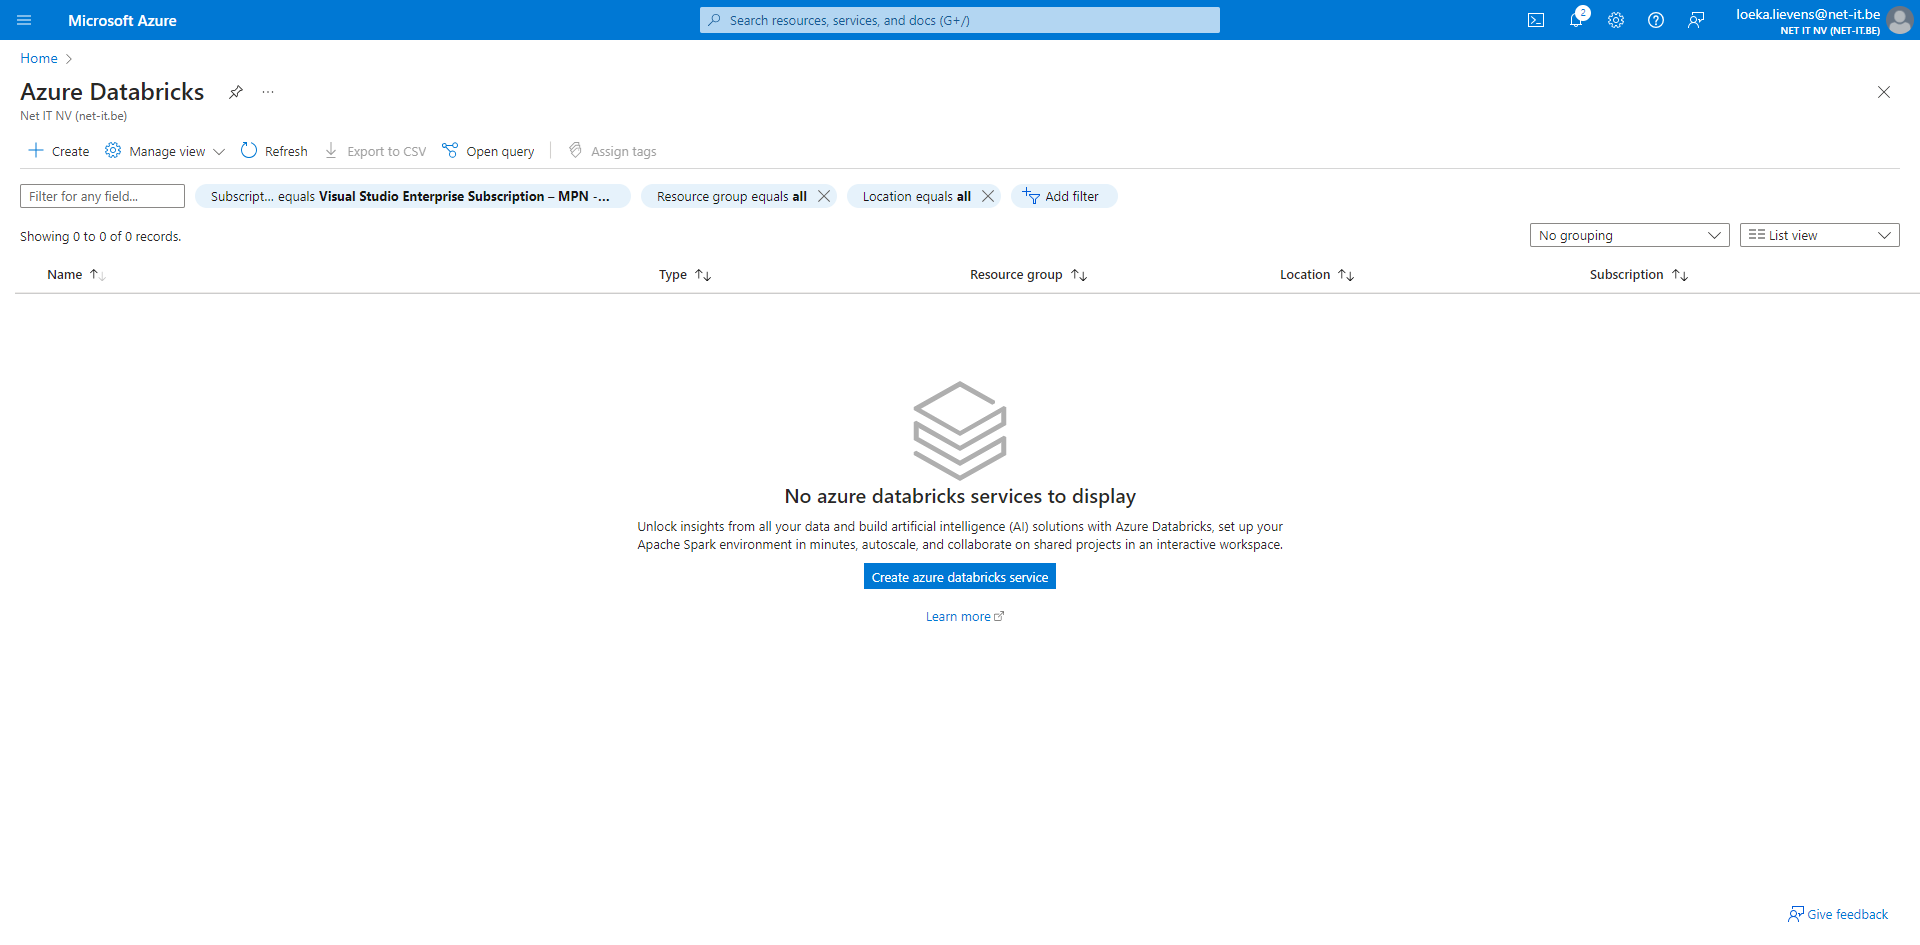
\includegraphics[width=0.9\textwidth]{./graphics/databricks/initial_1.png}
    \footnote{Aanmaken van Azure Databricks}
\end{center}

Door in Microsoft Azure naar Databricks te navigeren kunnen we een nieuwe Azure Databricks workspace gaan aanmaken.

\begin{center}
    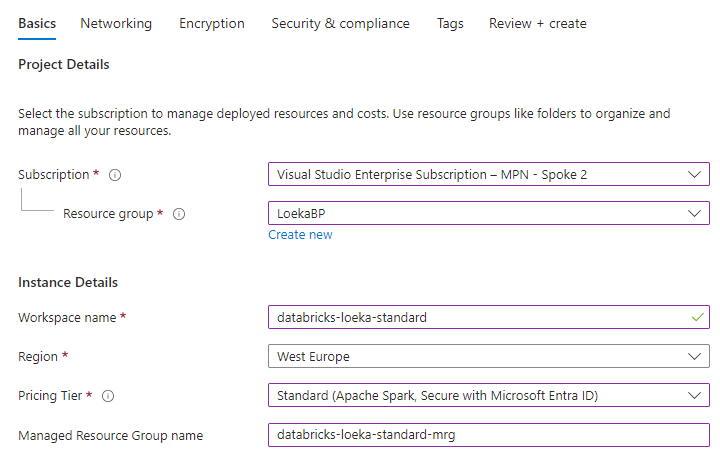
\includegraphics[width=0.6\textwidth]{./graphics/databricks/initial_2.png}
    \footnote{Configuratie van Azure Databricks}
\end{center}

Bij het aanmaken van databricks moet er een subscription en resource group gekozen worden. Er kan een nieuwe resource group aangemaakt worden of een reeds bestaande gekozen worden. Daarnaast moet er een naam, gewenste regio en pricing tier gekozen worden. Als pricing tier kiezen we hier voor Standard doordat we geen gebruik gaan maken van Premium features. Ten slotte kan er ook een Managed Resource Group name gekozen worden. Deze resource group houdt alle resource bij die databricks nodig heeft, zoals bijvoorbeeld virtual machines, storage accounts en virtual networks.

\begin{center}
    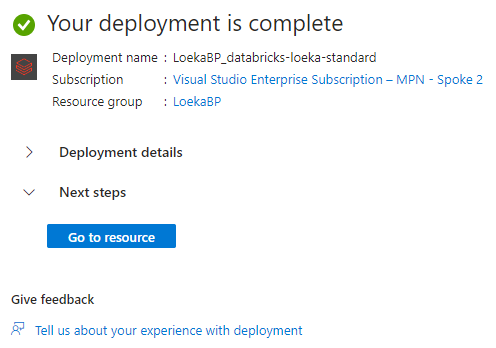
\includegraphics[width=0.6\textwidth]{./graphics/databricks/initial_3.png}
    \footnote{Deployment complete van Azure Databricks}
\end{center}

Wanneer de resource is aangemaakt kan Azure Databricks opgestart worden.

\begin{center}
    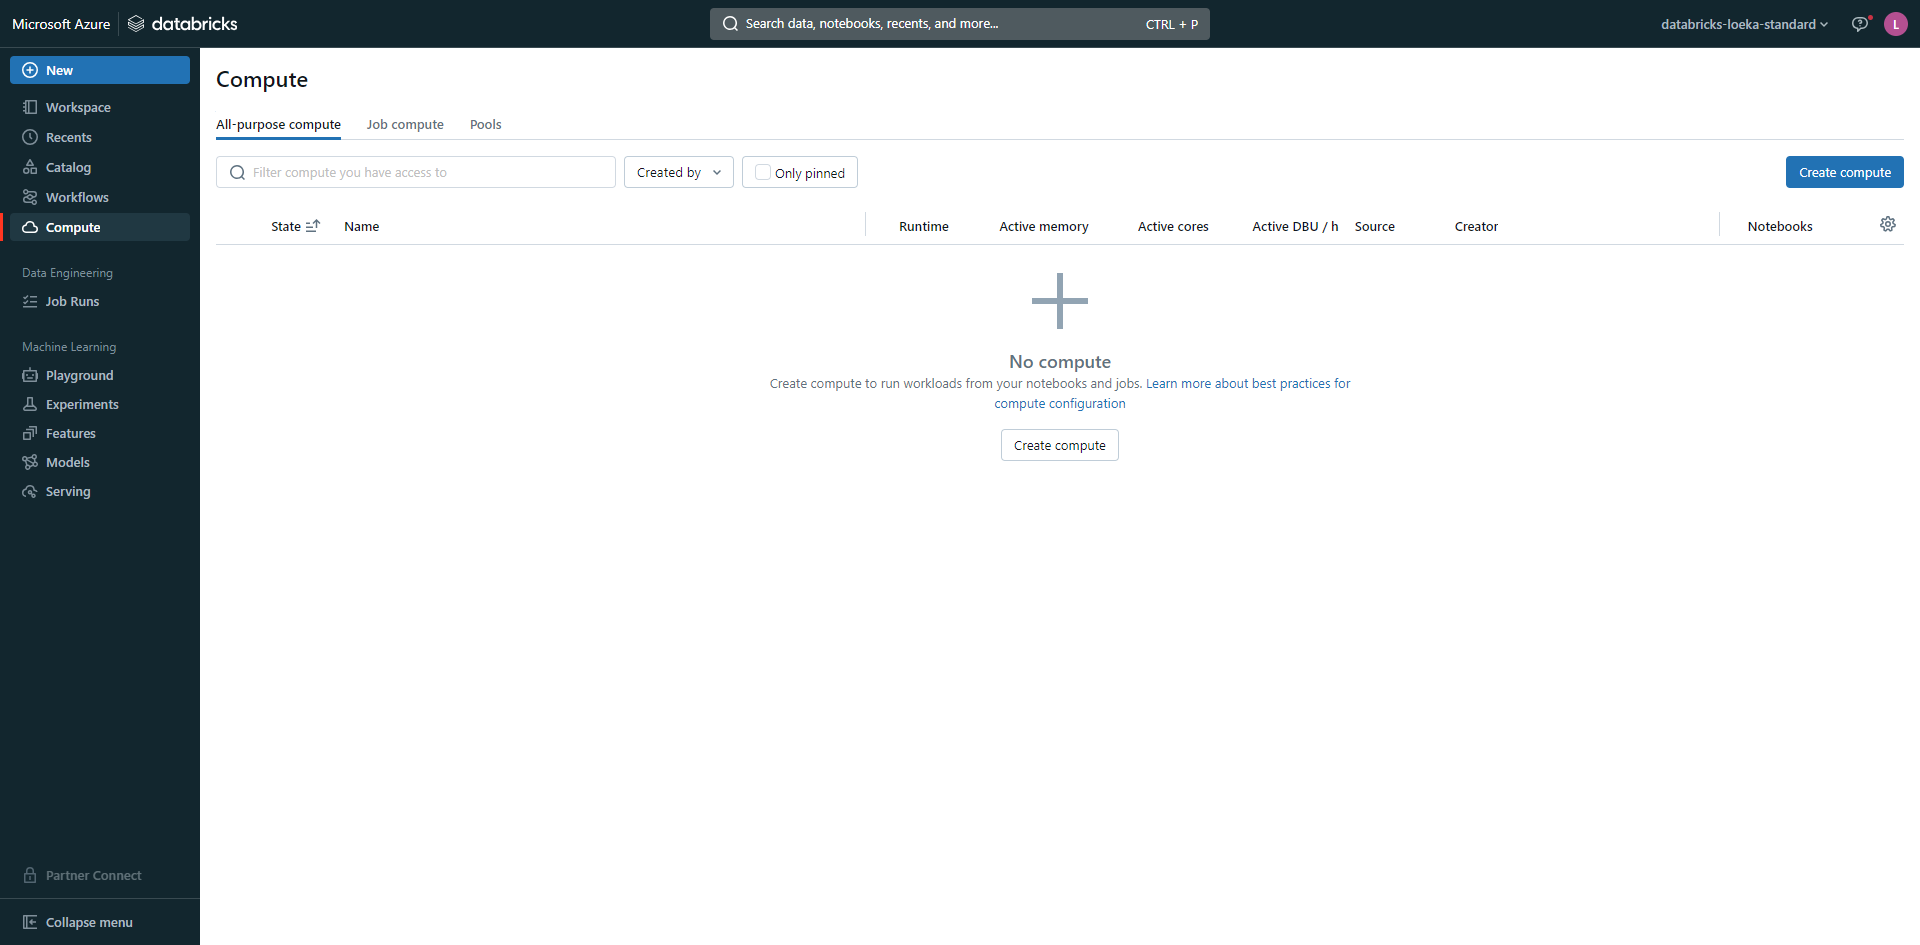
\includegraphics[width=0.9\textwidth]{./graphics/databricks/initial_4.png}
    \footnote{Aanmaken van compute resource}
\end{center}

Voor we notebooks en jobs gaan kunnen uitvoeren zullen we eerst een compute resource moeten gaan aanmaken.

\begin{center}
    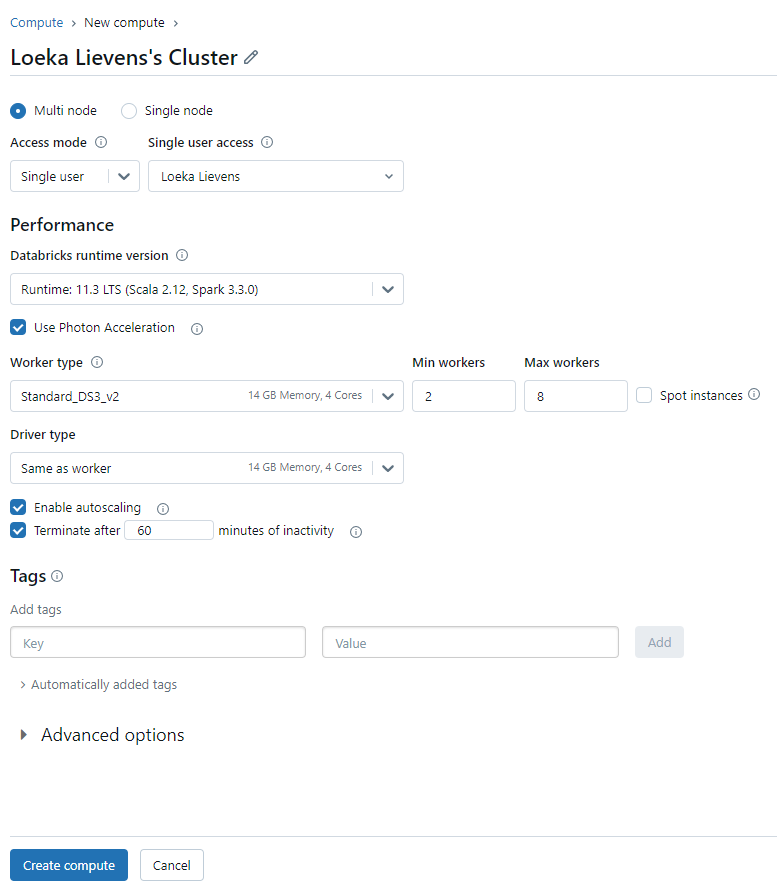
\includegraphics[width=0.6\textwidth]{./graphics/databricks/initial_5.png}
    \footnote{Configuratie van compute resource}
\end{center}

De databricks runtime version moet op 11.3 LTS gezet worden zodat we Apache Spark 3.3.0 kunnen gebruiken. Dit omdat we gebruik gaan maken van `spark-cdm-connector`. Ook hebben we ingesteld dat de cluster zichzelf zal uitschakelen na 60 minuten om onnodige kosten te voorkomen.

\begin{center}
    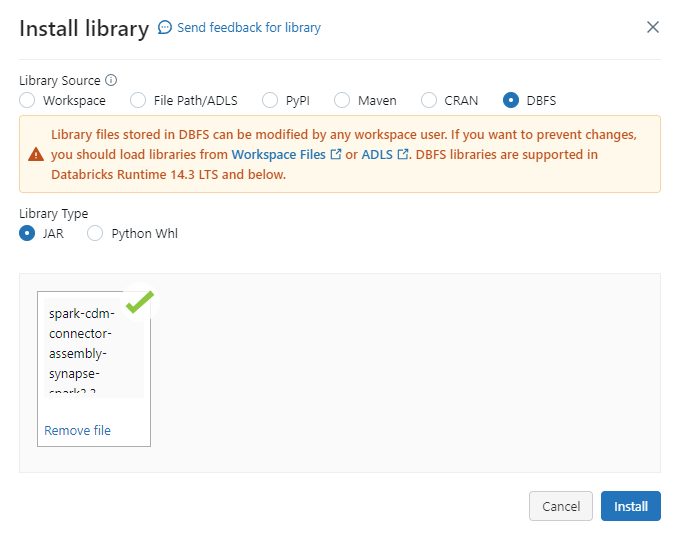
\includegraphics[width=0.9\textwidth]{./graphics/databricks/initial_6.png}
    \footnote{Installatie van `spark-cdm-connector`}
\end{center}

Ten slotte moet de \href{https://github.com/Azure/spark-cdm-connector/releases/tag/spark3.3-1.19.5}{jar file} van `spark-cdm-connector` geïnstalleerd worden in het aangemaakte compute resource om gebruik te kunnen maken van het Common Data Model in onze pipeline.

\subsection{Collaboration en source control}

Databricks folders is een visuele Git client binnen Azure Databricks om gebruik te kunnen maken van source control.

\begin{center}
    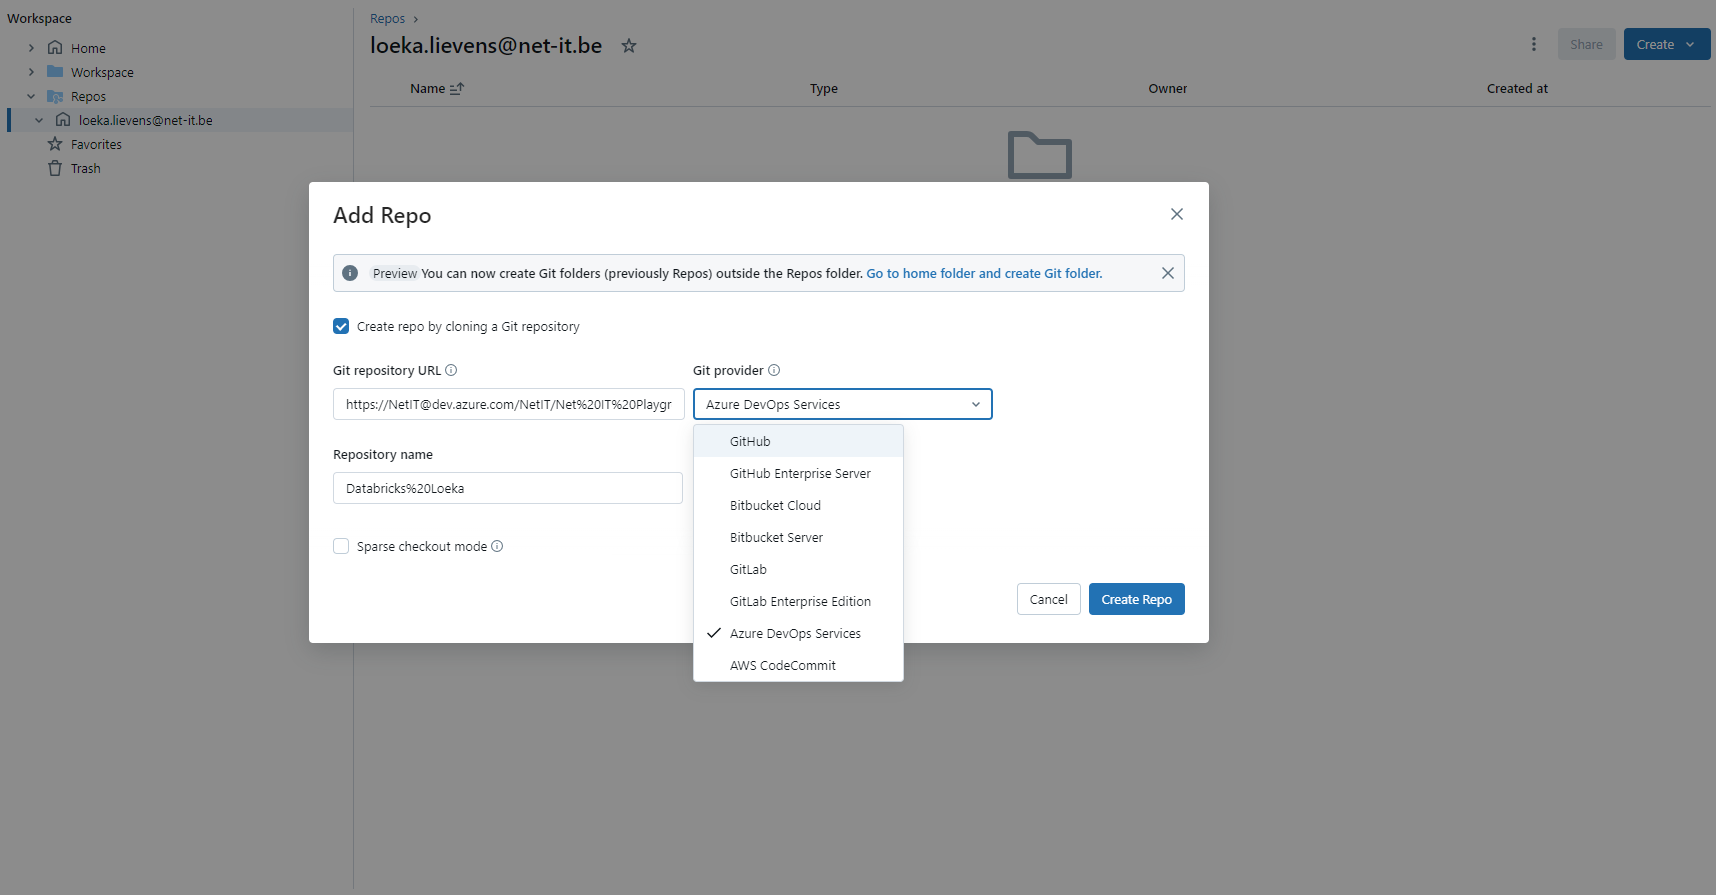
\includegraphics[width=0.9\textwidth]{./graphics/databricks/git_1.png}
    \footnote{Clone Git repository in Databricks folders}
\end{center}

Het geeft de optie om verschillende Git providers te gaan gebruiken. Doordat er binnen Net IT gewerkt wordt met Azure DevOps Services zal hier voor gekozen worden.

\begin{center}
    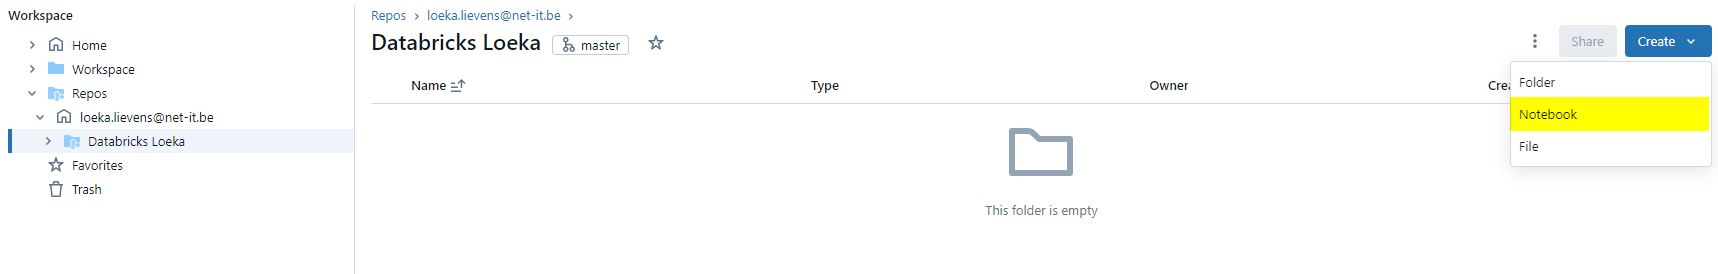
\includegraphics[width=0.9\textwidth]{./graphics/databricks/git_2.png}
    \footnote{Aanmaken van een notebook in databricks}
\end{center}

Ter illustratie zal er een voorbeeld notebook aangemaakt worden.

\begin{center}
    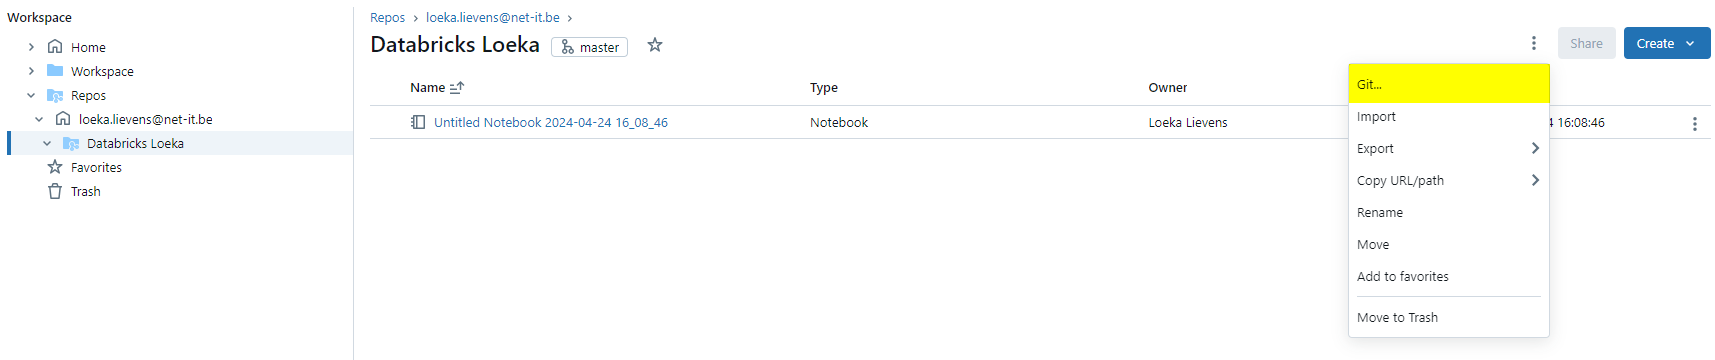
\includegraphics[width=0.9\textwidth]{./graphics/databricks/git_3.png}
    \footnote{Commit en push in Databricks}
\end{center}

\begin{center}
    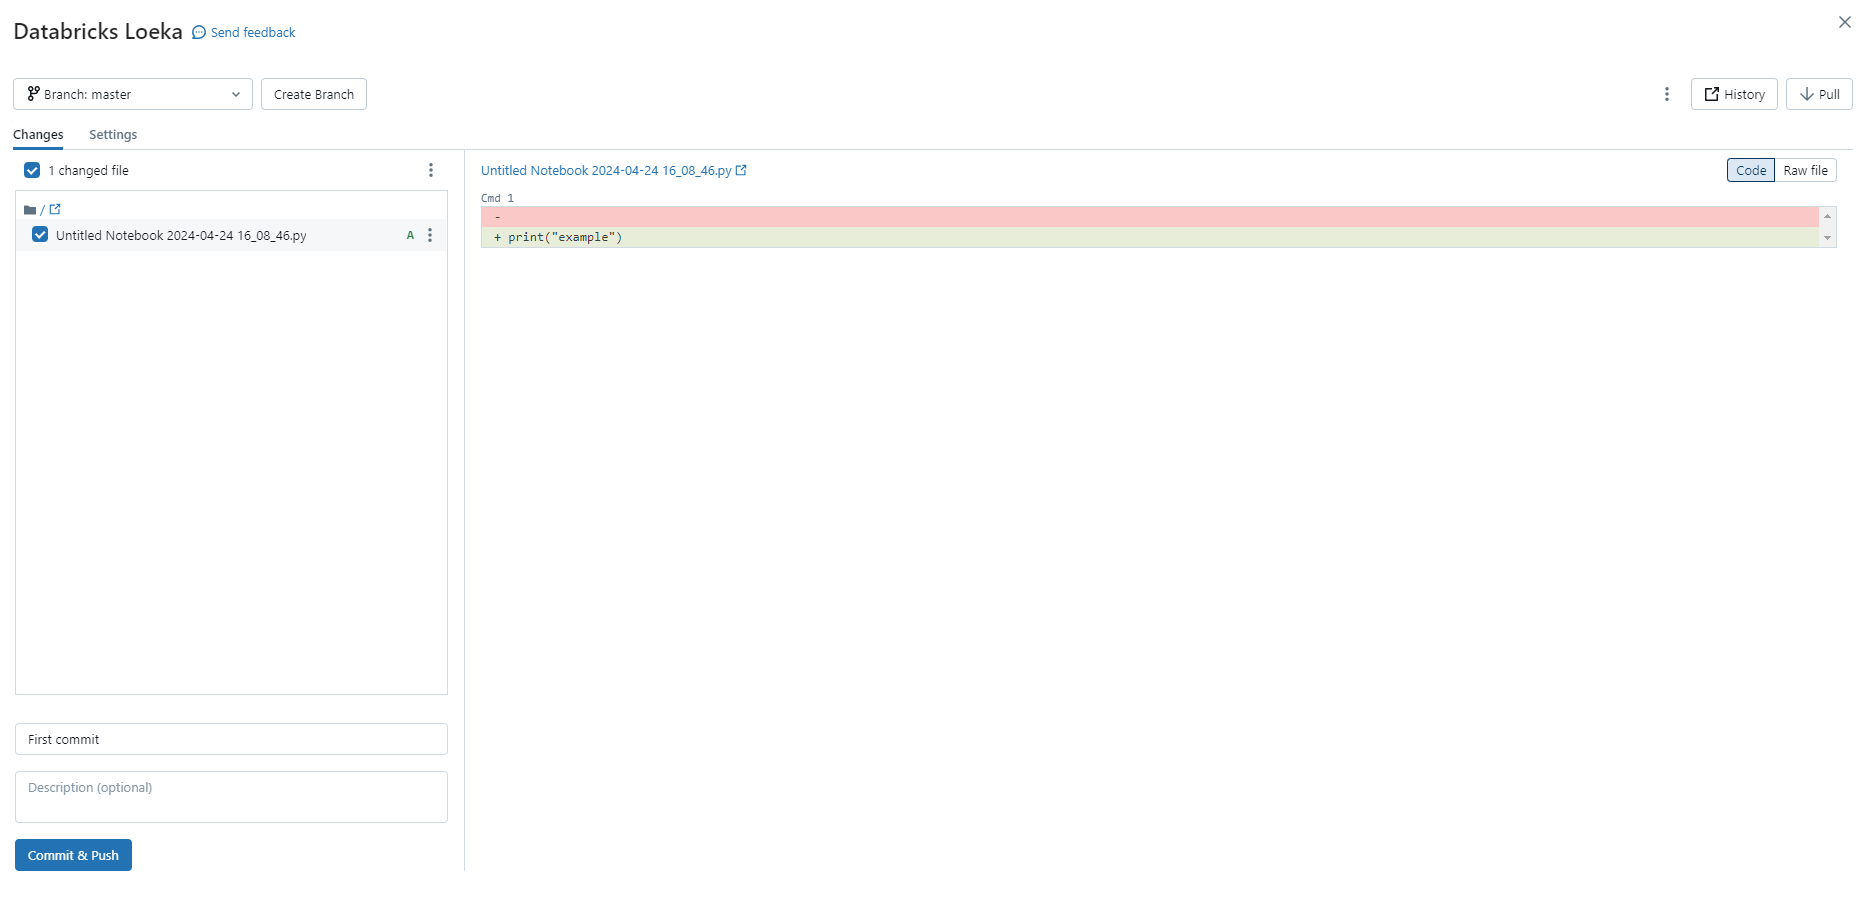
\includegraphics[width=0.9\textwidth]{./graphics/databricks/git_4.png}
    \footnote{Commit en push in Databricks}
\end{center}

Deze notebook kan dan gecommit worden naar Git.

% Einde nieuw

%\begin{center}
%    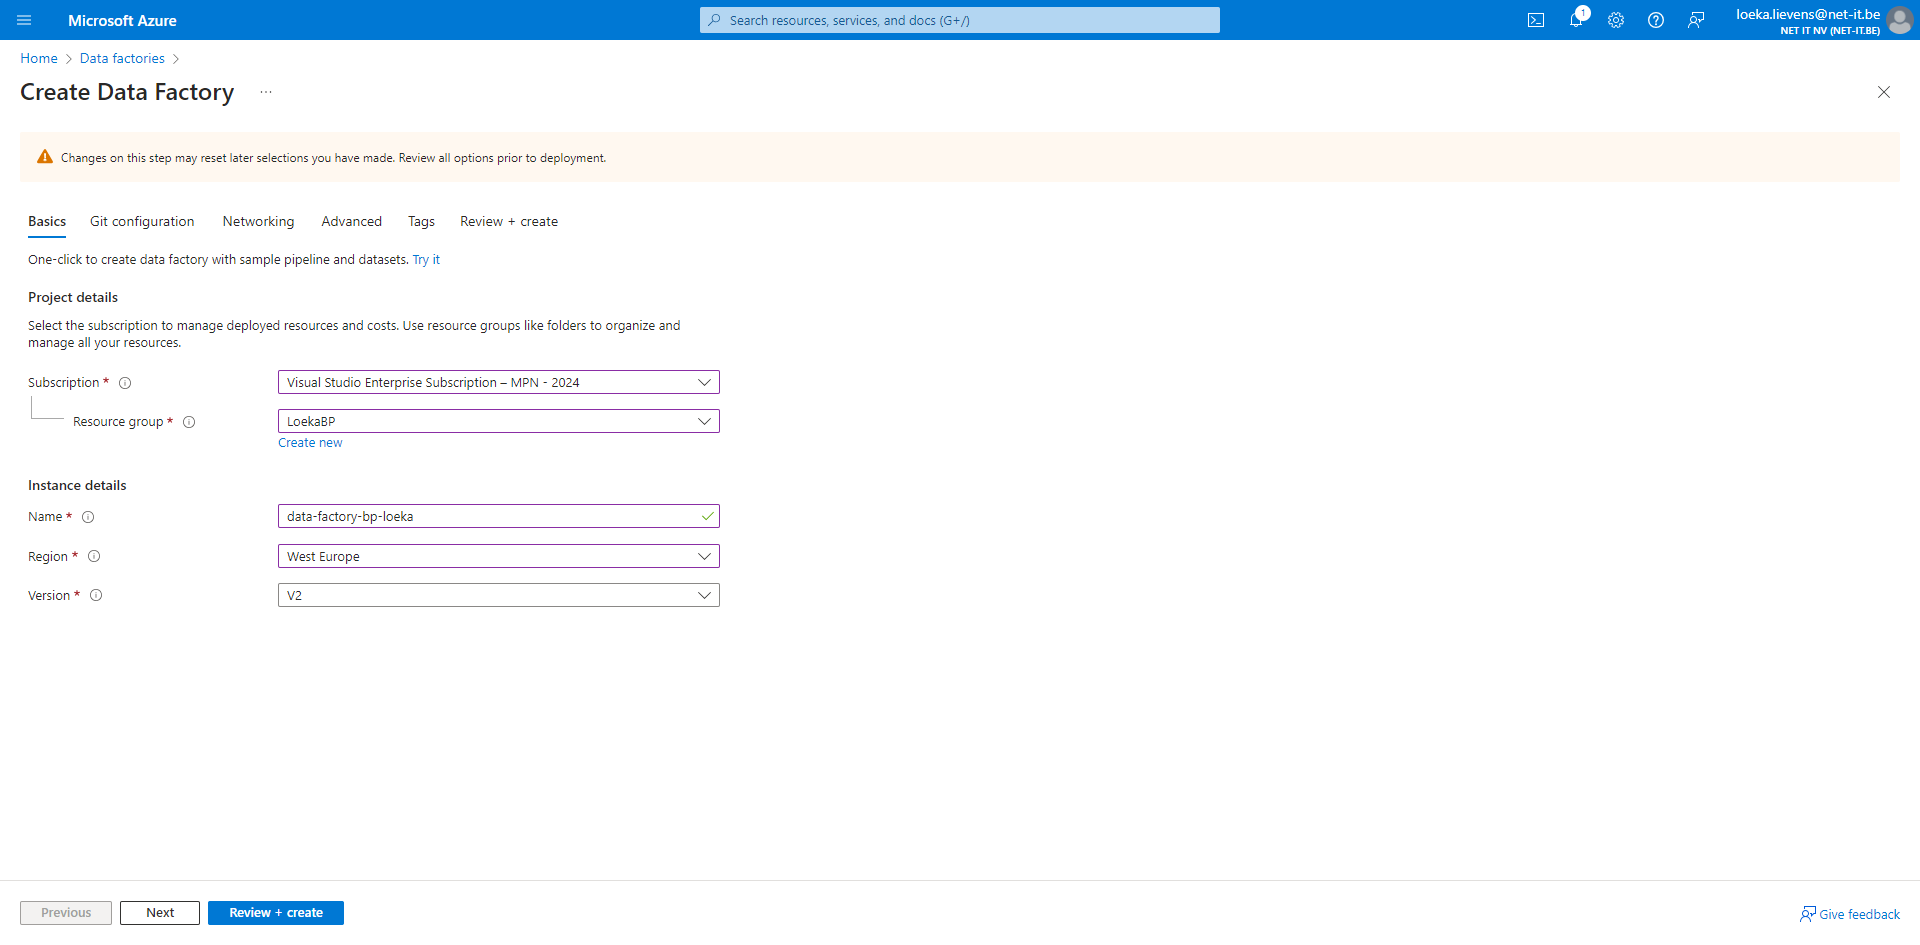
\includegraphics[width=1\textwidth]{./graphics/adf/initial_1.png}
%\end{center}
%
%Selecteer een gewenste subsscription en resource group. Er kan gekozen worden voor een resource group die er al bestaat of om een nieuwe aan te maken. Hier na kan er een naam en gewenste regio gekozen worden. De version laten we staan op V2.
%
%\begin{center}
%    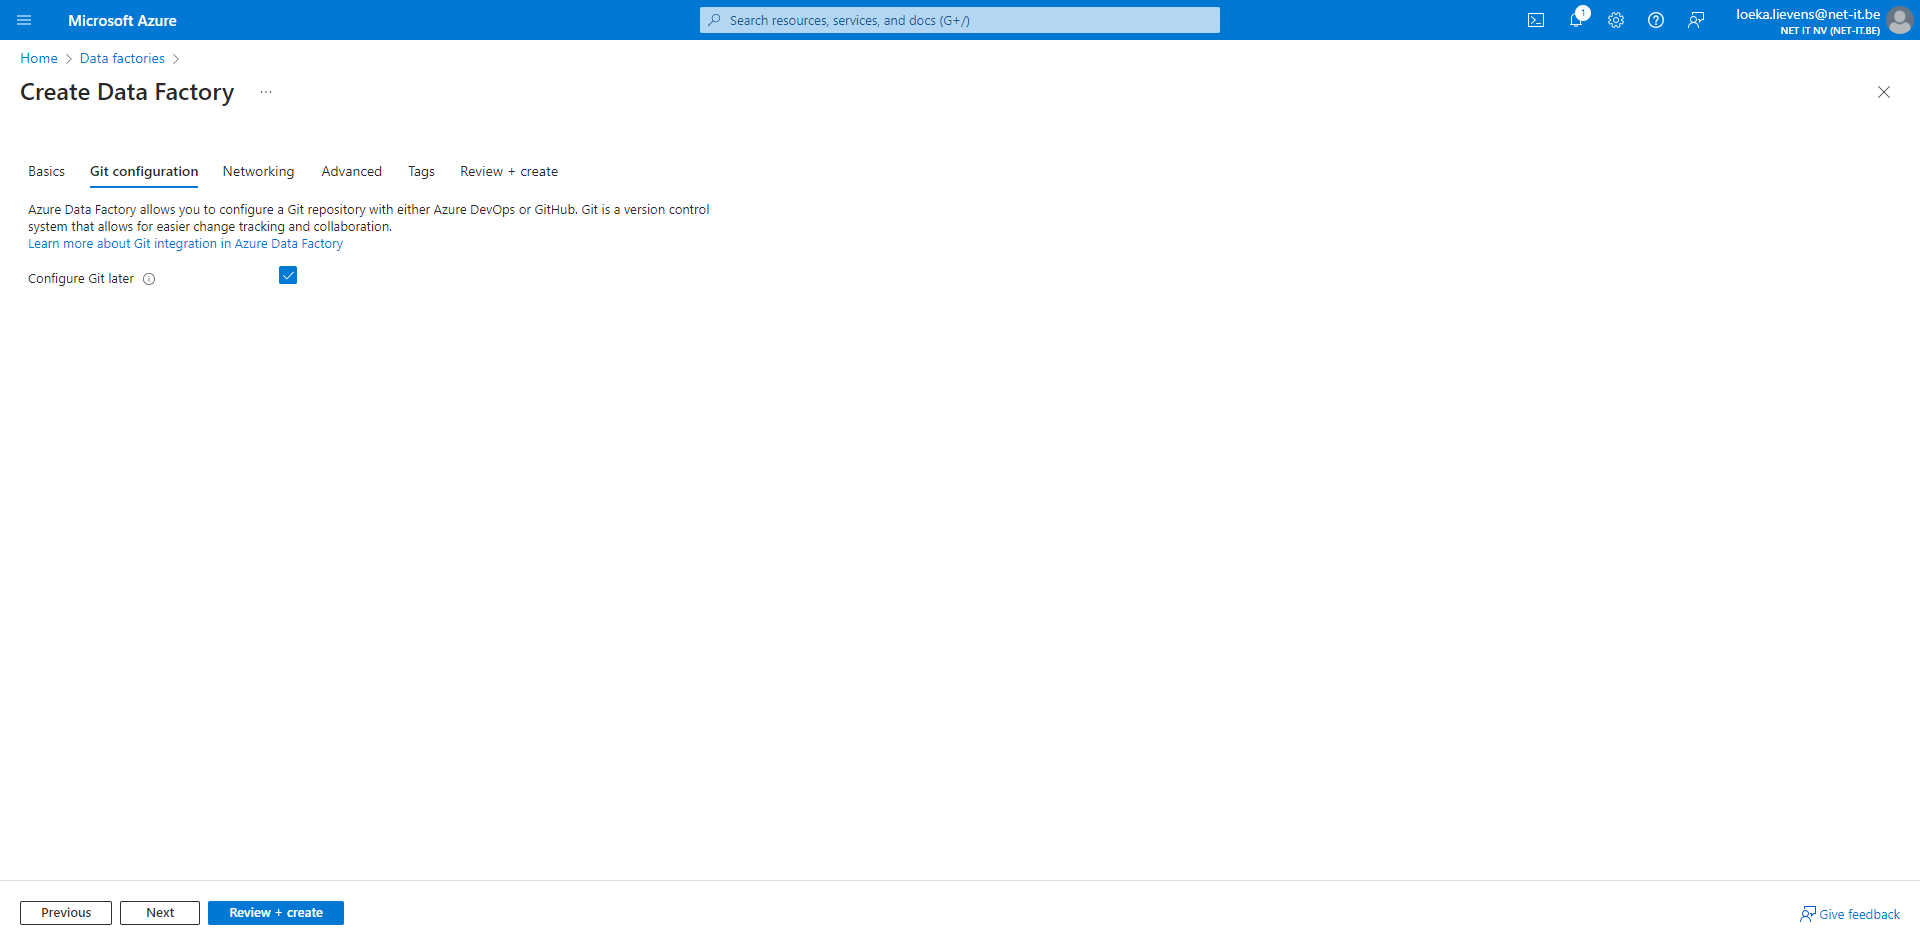
\includegraphics[width=1\textwidth]{./graphics/adf/initial_2.png}
%\end{center}
%
%Door bij de vorige stap op next te klikken kunnen we er voor kiezen om een Git configuratie te gaan toevoegen. Dit zullen we pas later gaan doen. Klik nu op `Review + create` om de data factory aan te maken.
%
%\begin{center}
%    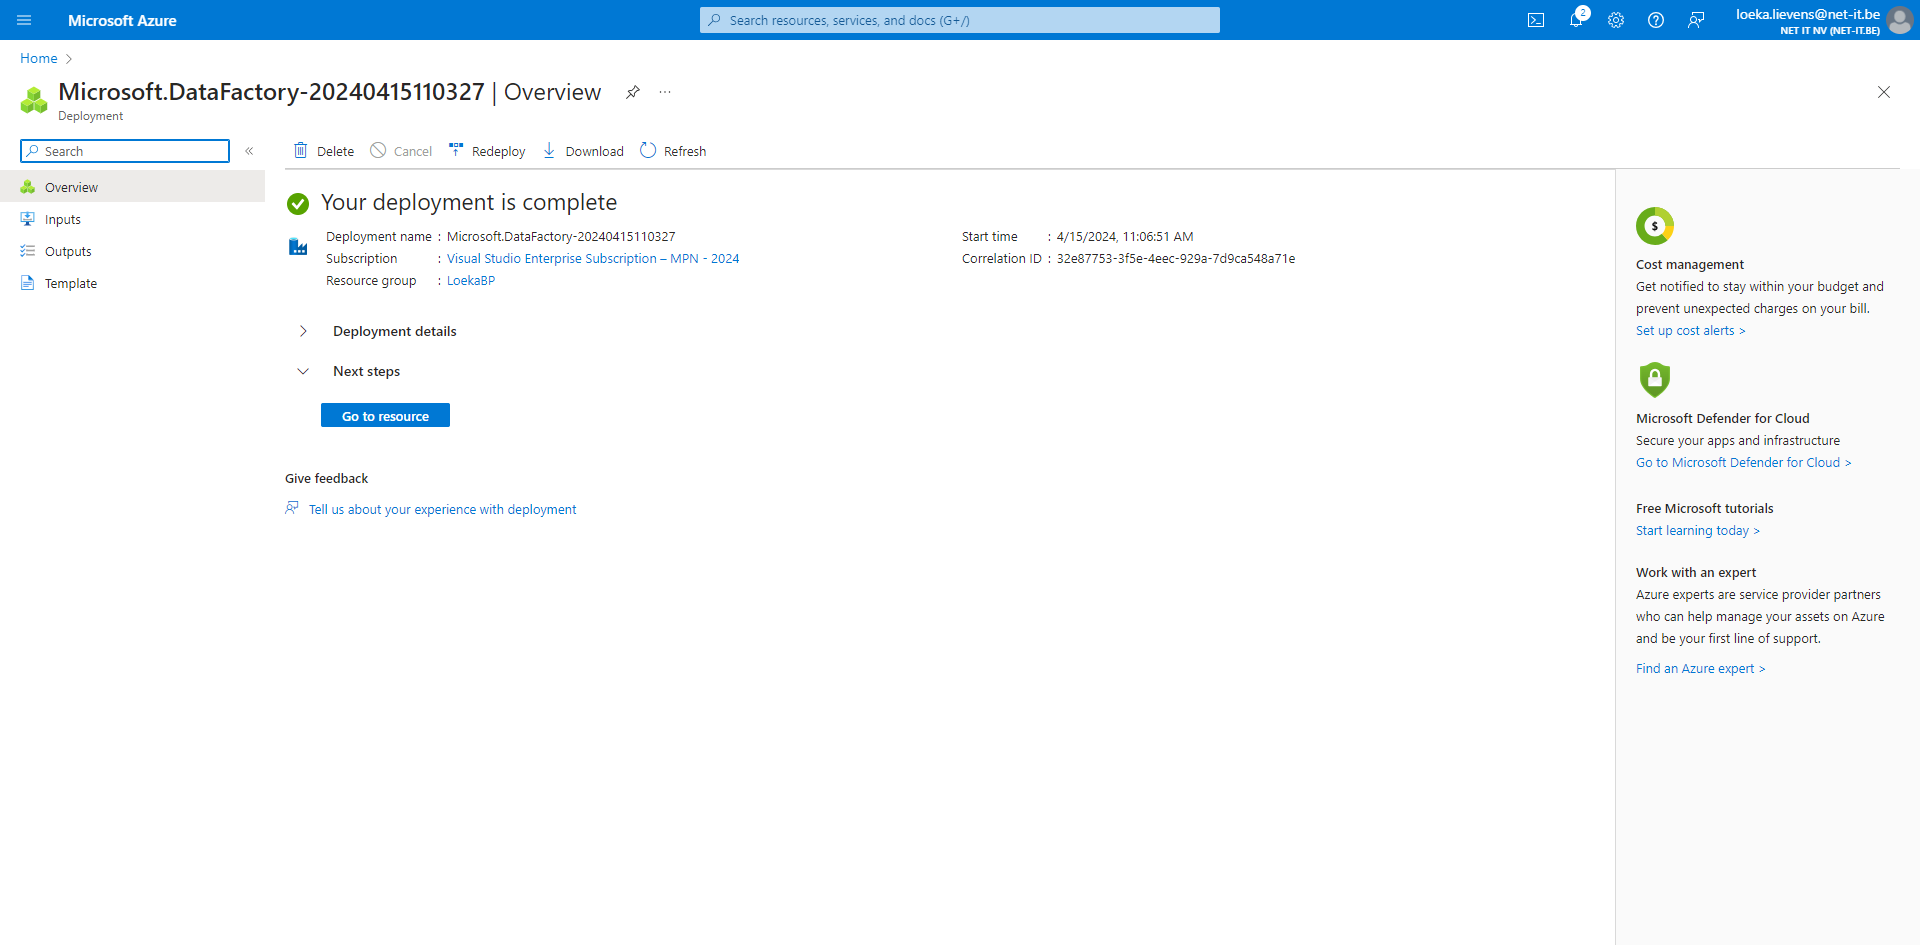
\includegraphics[width=1\textwidth]{./graphics/adf/deployment_complete.png}
%\end{center}
%
%Wanneer onze deployment complete is kunnen we naar onze resource gaan door op `Go to resource` te klikken.
%
%\begin{center}
%    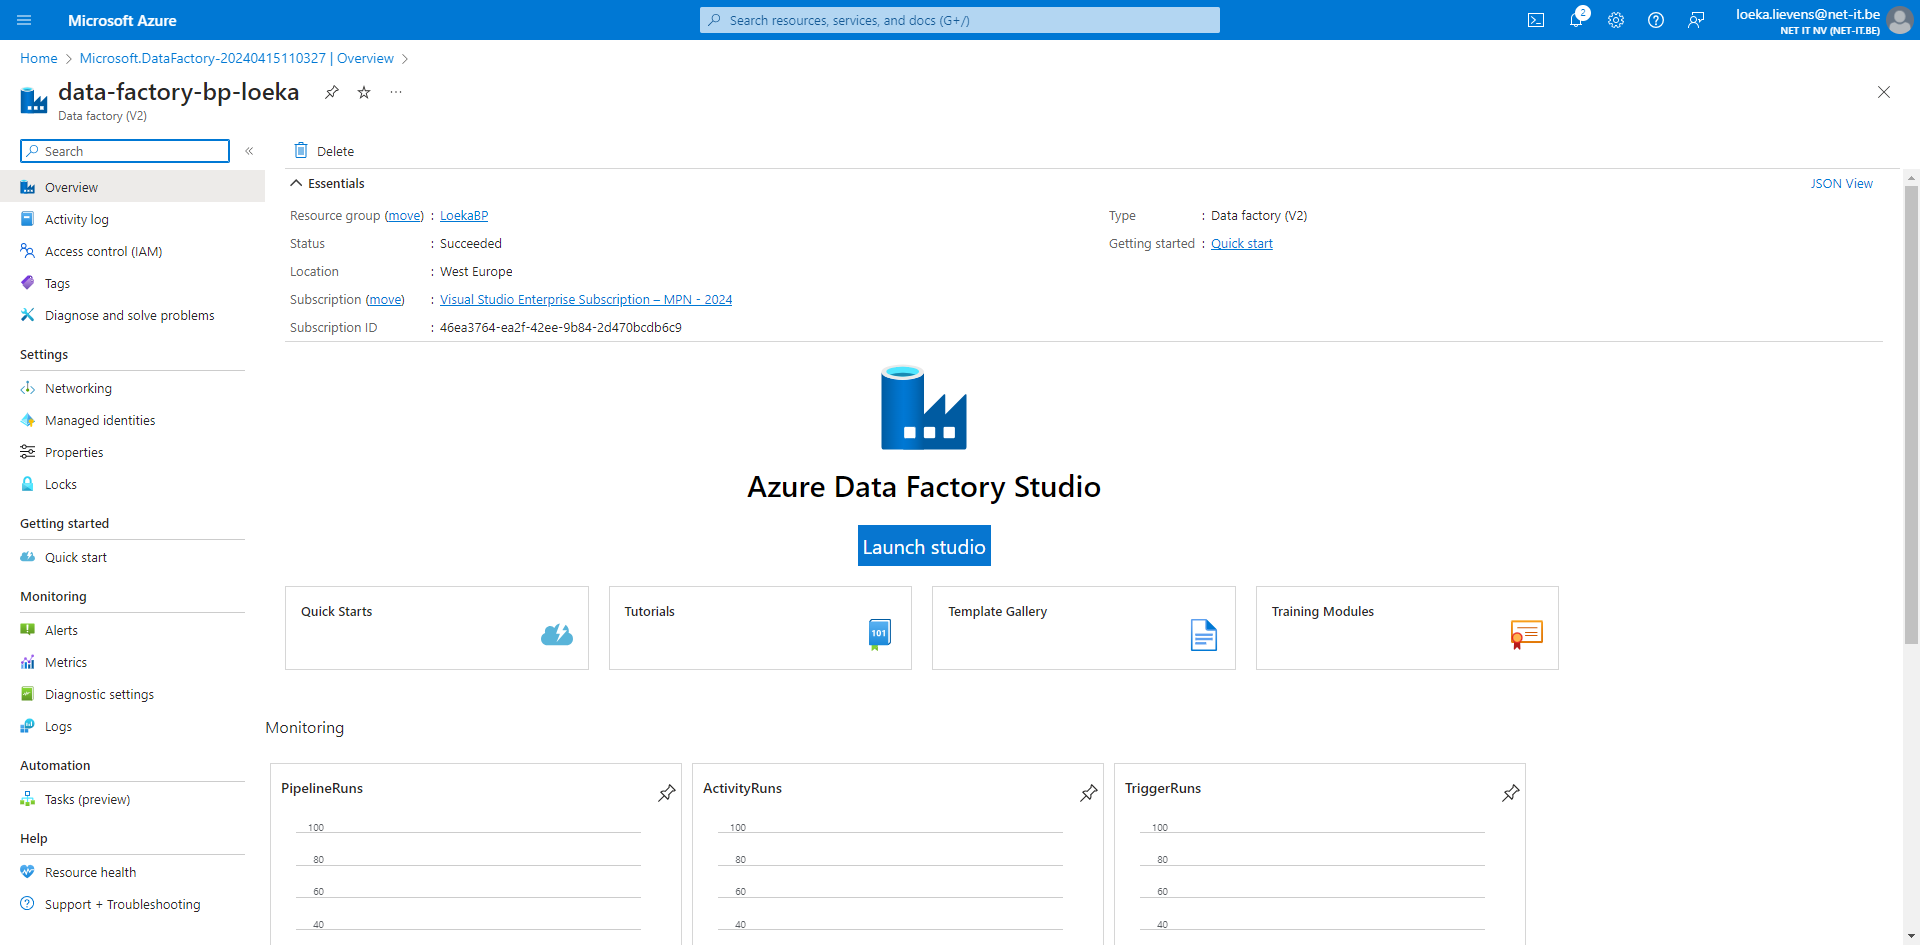
\includegraphics[width=1\textwidth]{./graphics/adf/launch_adf.png}
%\end{center}
%
%Klik nu op `Launch studio` om naar Azure Data Factory Studio te gaan.
%
%\subsubsection{Koppeling met Git}
%
%\begin{center}
%    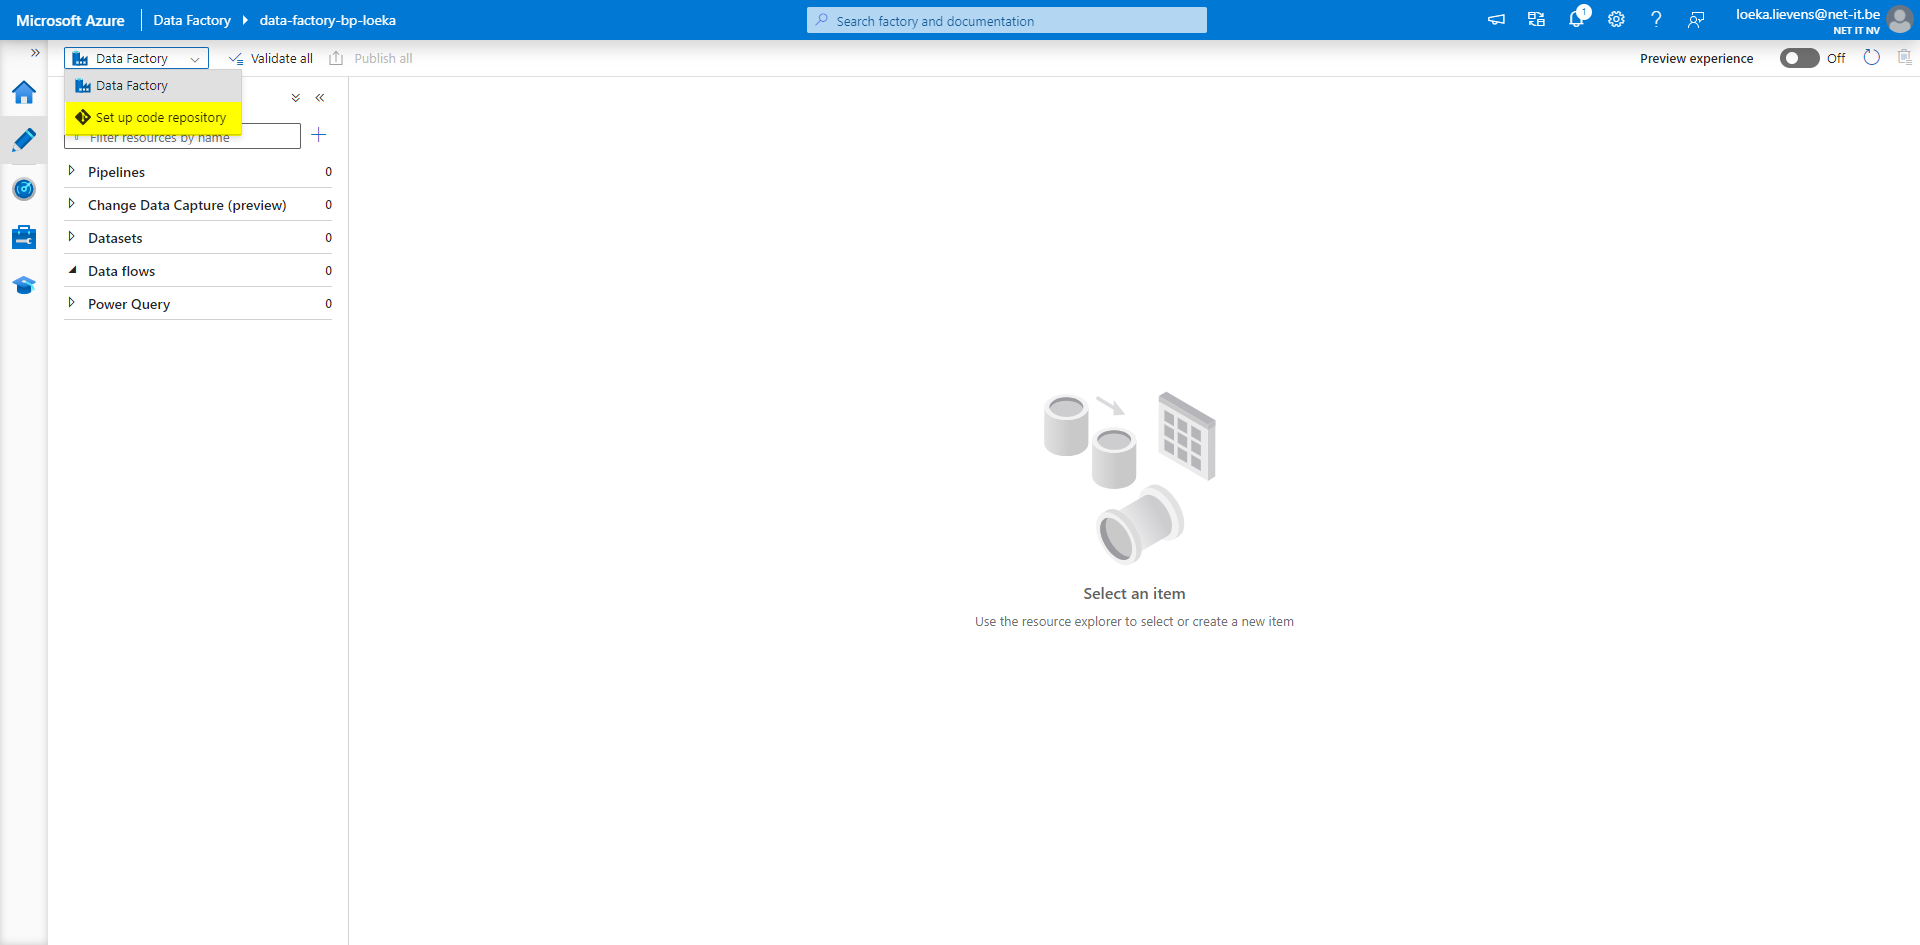
\includegraphics[width=1\textwidth]{./graphics/adf/setup_repository.png}
%\end{center}
%
%Voor we onze ETL gaan implementeren zullen we eerst onze data factory koppelen met Git.
%
%\begin{center}
%    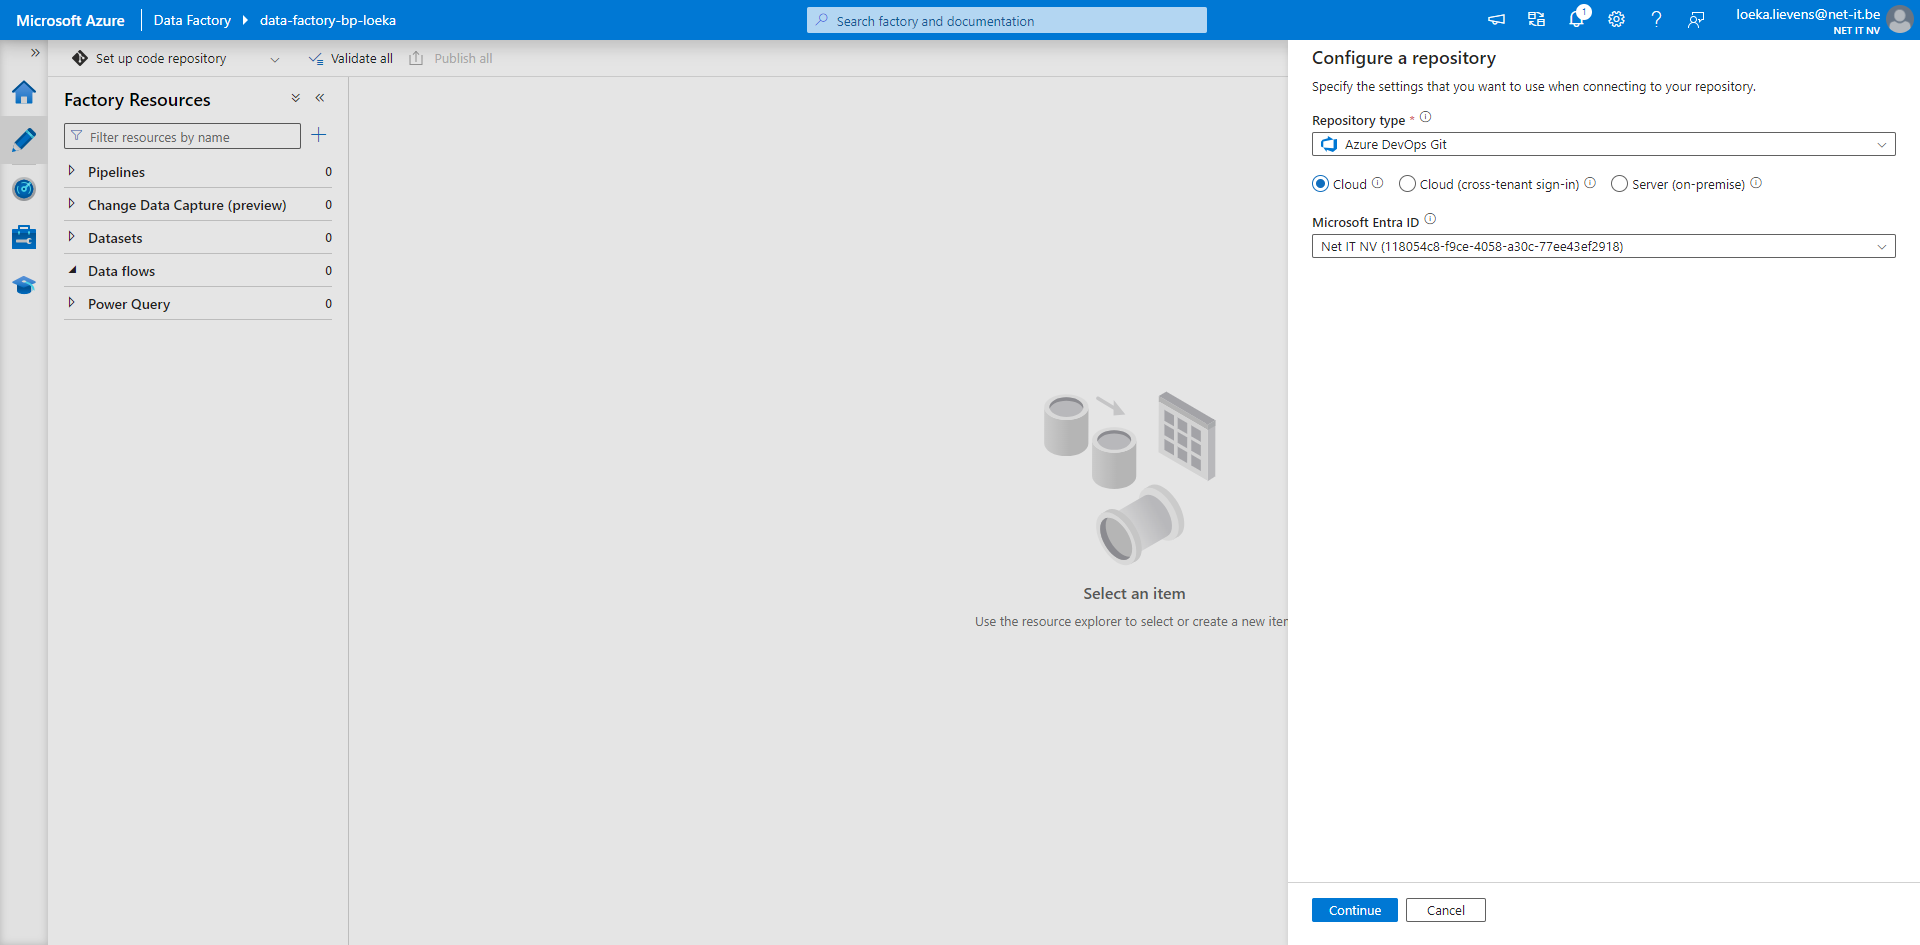
\includegraphics[width=1\textwidth]{./graphics/adf/setup_repository_2.png}
%\end{center}
%
%\begin{center}
%    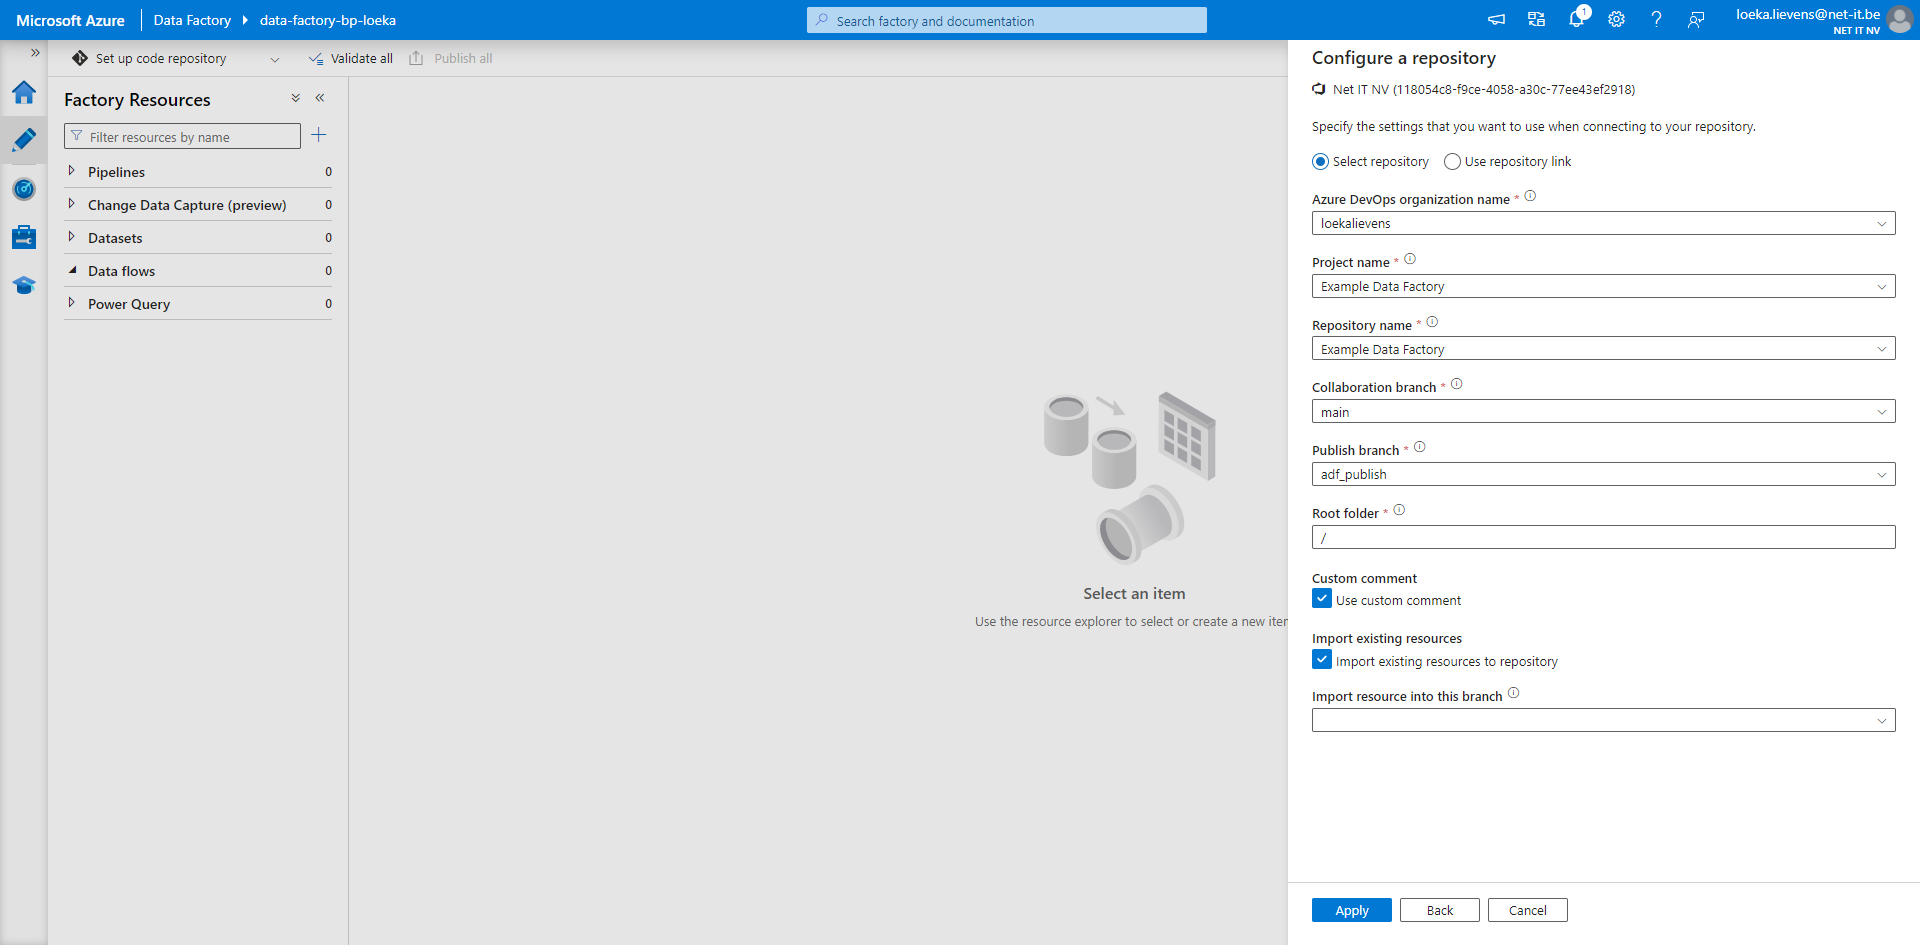
\includegraphics[width=1\textwidth]{./graphics/adf/setup_repository_3.png}
%\end{center}
%
%Binnen Net IT wordt er gewerkt met Azure DevOps Git.
%
%\subsubsection{Het toevoegen van een source}
%
%Telkens wanneer we een source tabel zullen gaan toevoegen zal dit op dezelfde manier gebeuren.
%
%\begin{center}
%    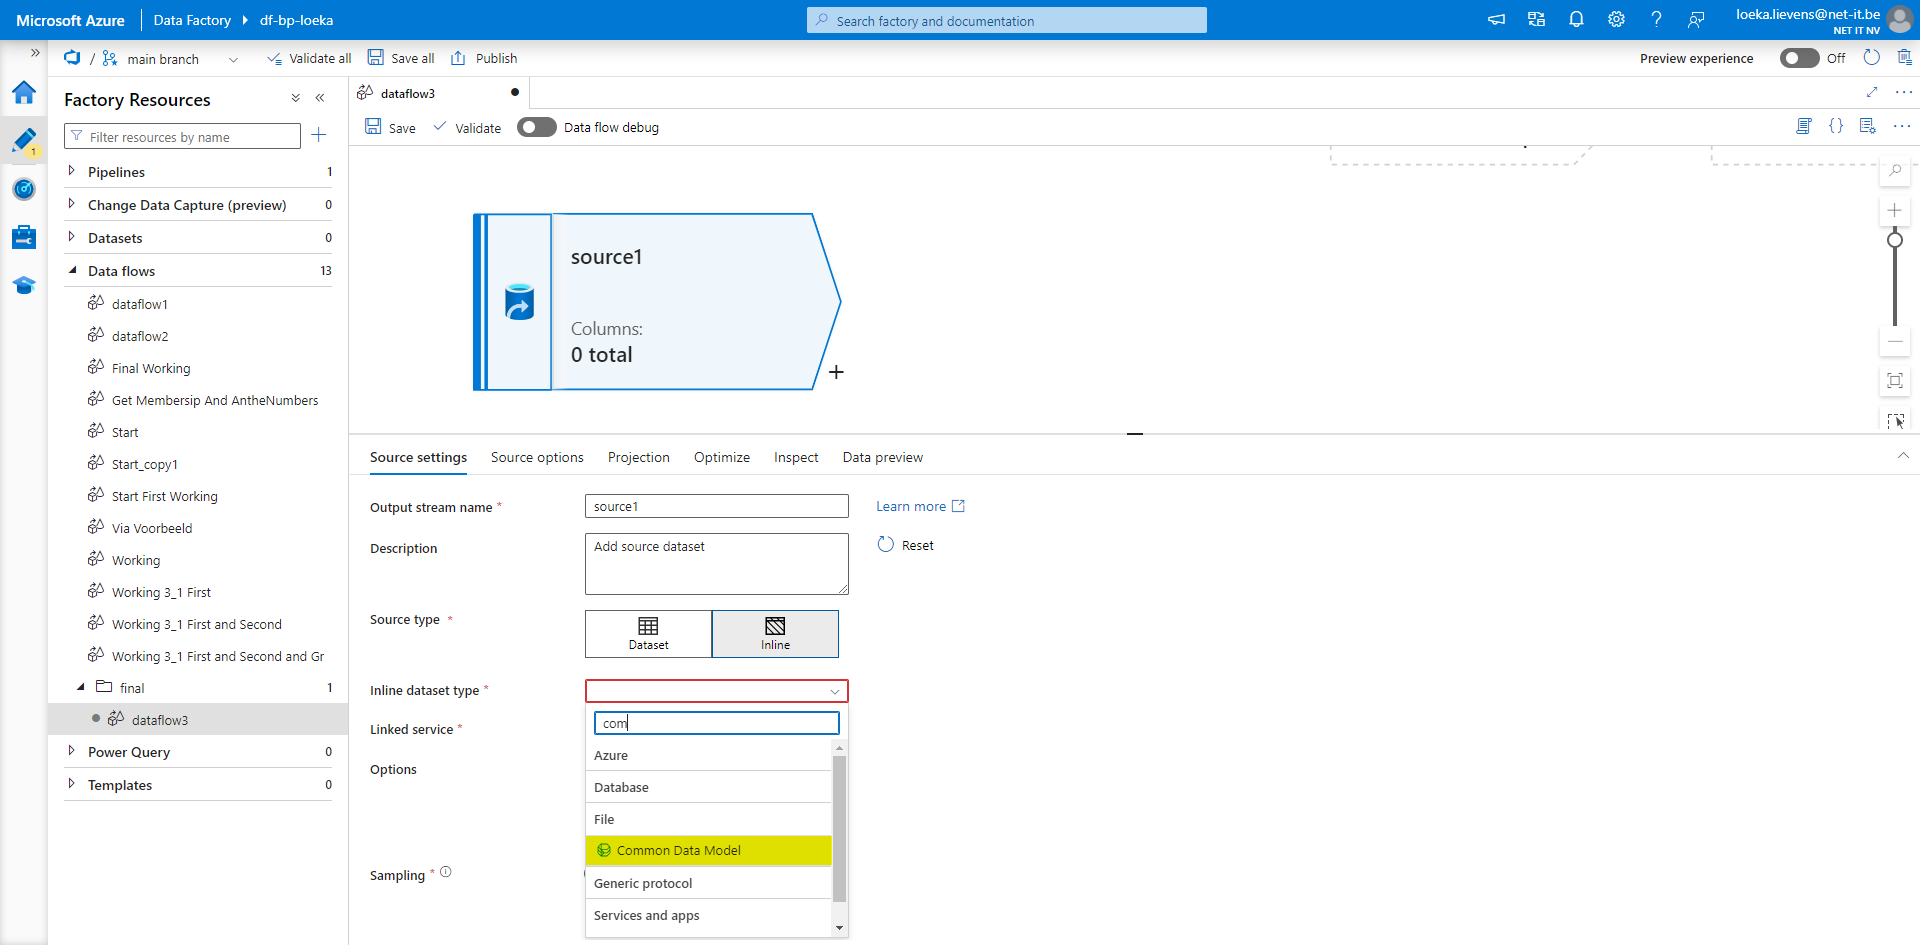
\includegraphics[width=1\textwidth]{./graphics/adf/source_table_1.png}
%\end{center}
%
%Als source type zal er steeds gekozen worden voor inline. Dit doordat we slechts één enkele dataflow zullen gaan aanmaken en geen gedeelde datasets nodig hebben. Als type voor de linked service kiezen we voor Common Data Model.
%
%\begin{center}
%    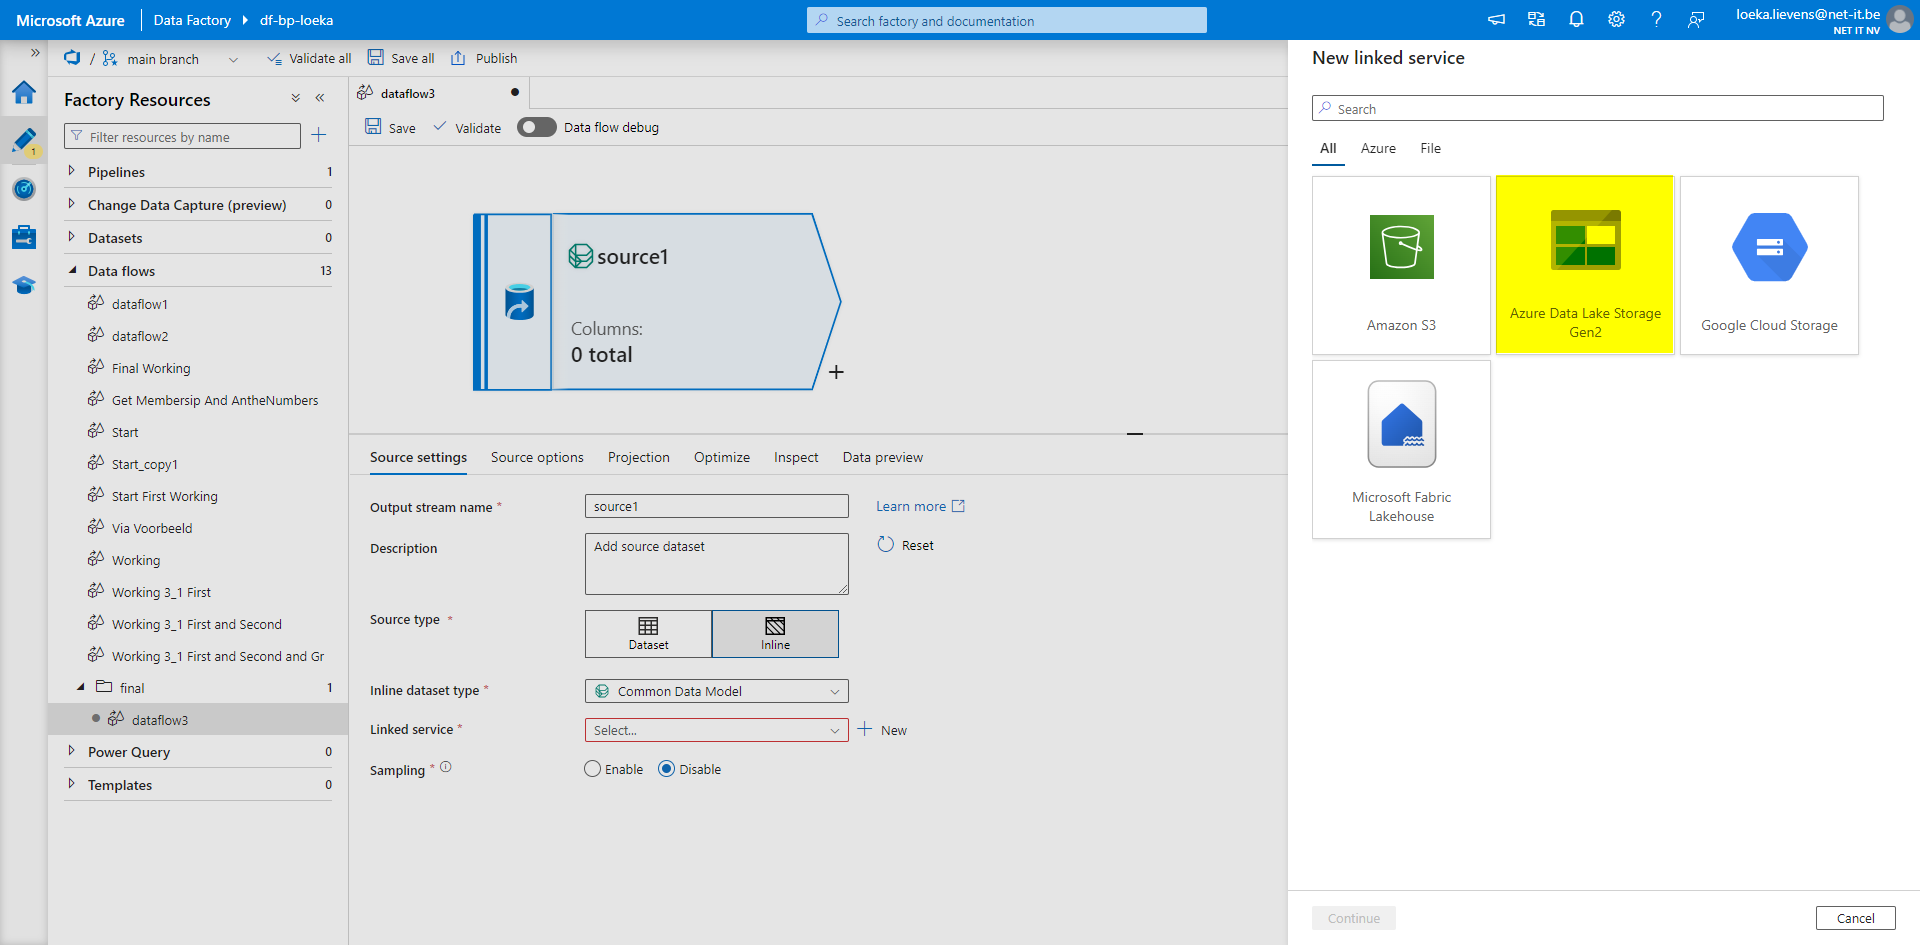
\includegraphics[width=1\textwidth]{./graphics/adf/source_table_2.png}
%\end{center}
%
%Er zal éénmalig een Linked Service aangemaakt moeten worden. Hierbij kiezen we voor Azure Data Lake Storage Gen2.
%
%\begin{center}
%    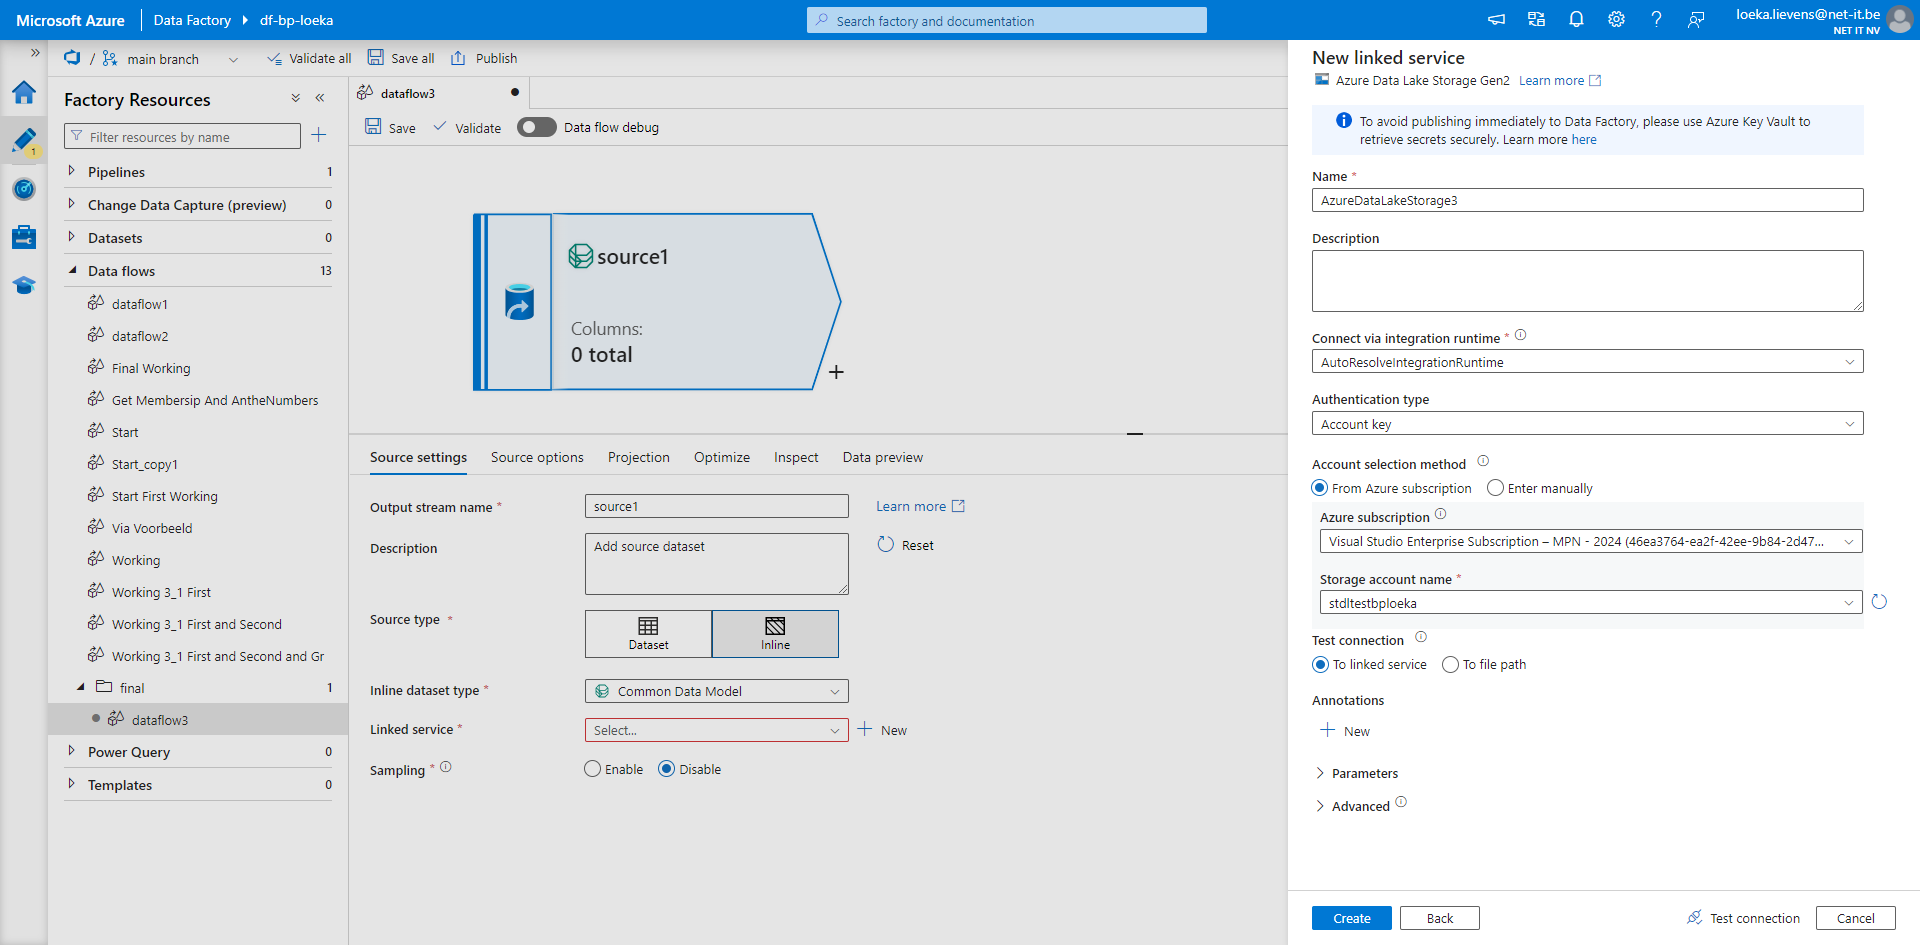
\includegraphics[width=1\textwidth]{./graphics/adf/source_table_3.png}
%\end{center}
%
%We kunnen makkelijk gaan koppelen met de juiste data lake door een Azure Subscription en Storage account name aan te duiden. Door op `Test connection` te klikken kunnen we kijken of de connectie met data lake is gelukt. Door op `Create` te klikken hebben we nu een Linked Service die steeds bij elke Source gebruikt kan worden.
%
%\begin{center}
%    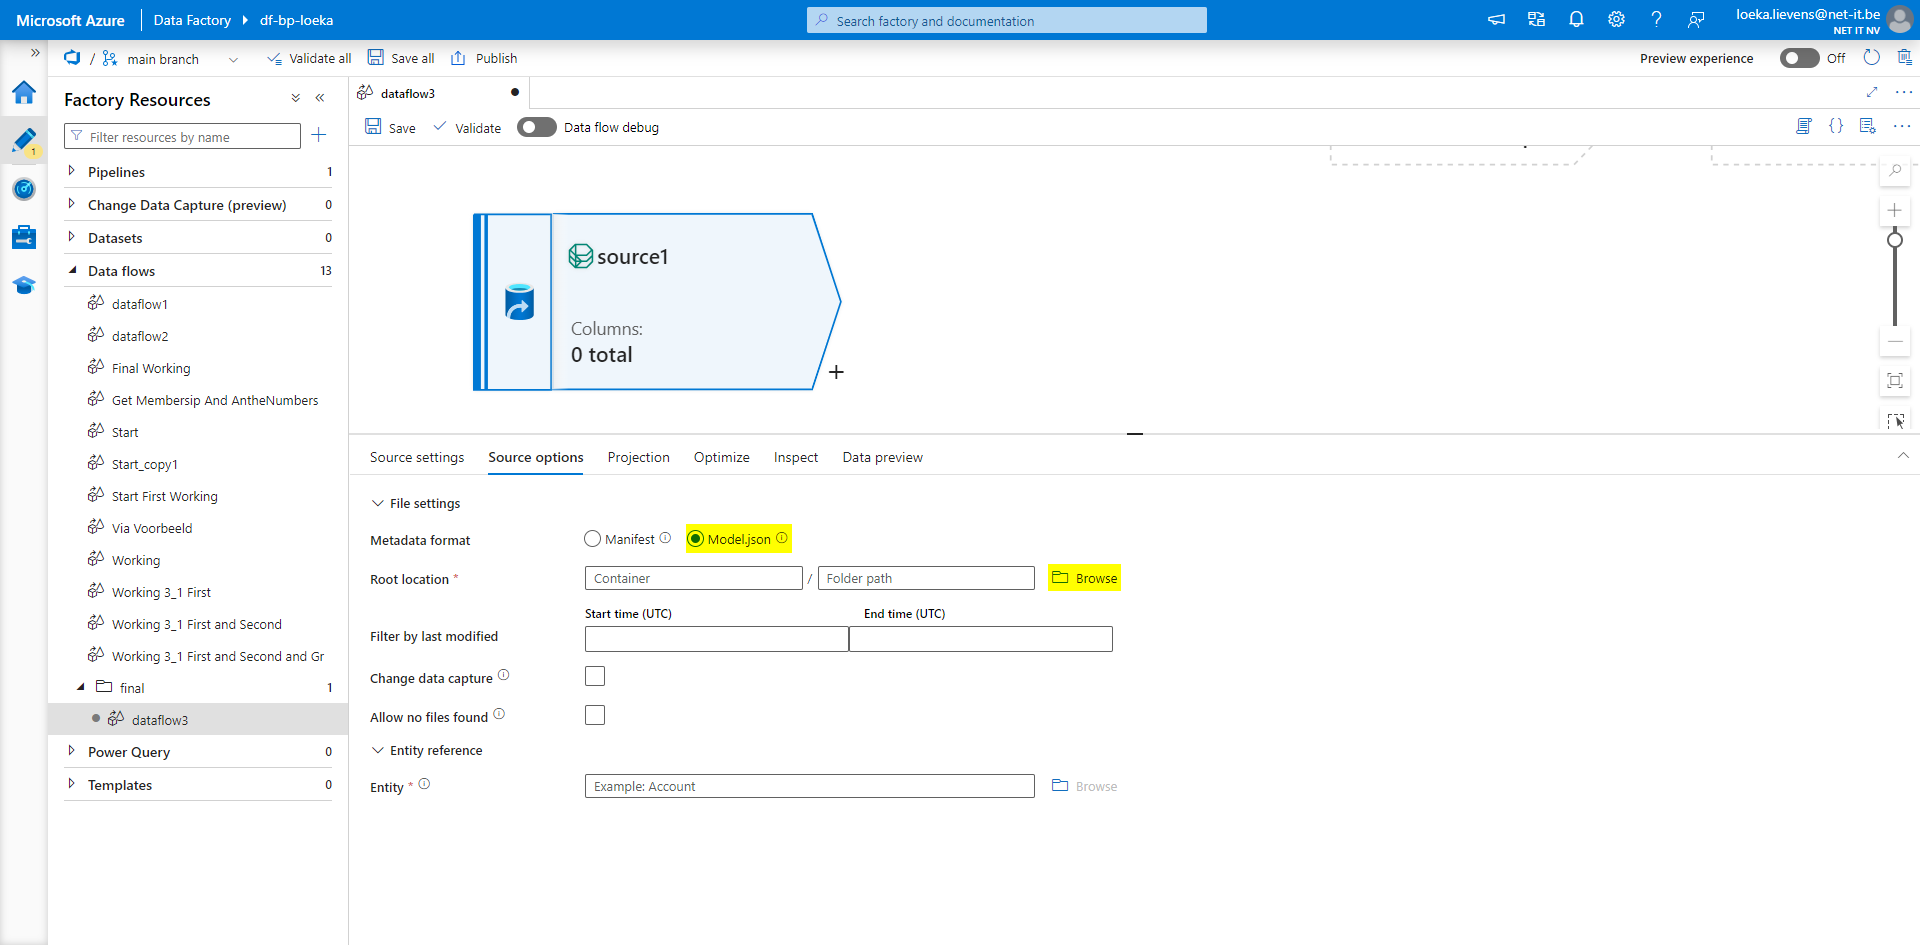
\includegraphics[width=1\textwidth]{./graphics/adf/source_table_4.png}
%\end{center}
%
%Door naar `Source options` te gaan kunnen we `Model.json` gaan aanduiden. Door op `Browse` te klikken kunnen we aanduiden waar het Model.json bestand te vinden is in data lake.
%
%\begin{center}
%    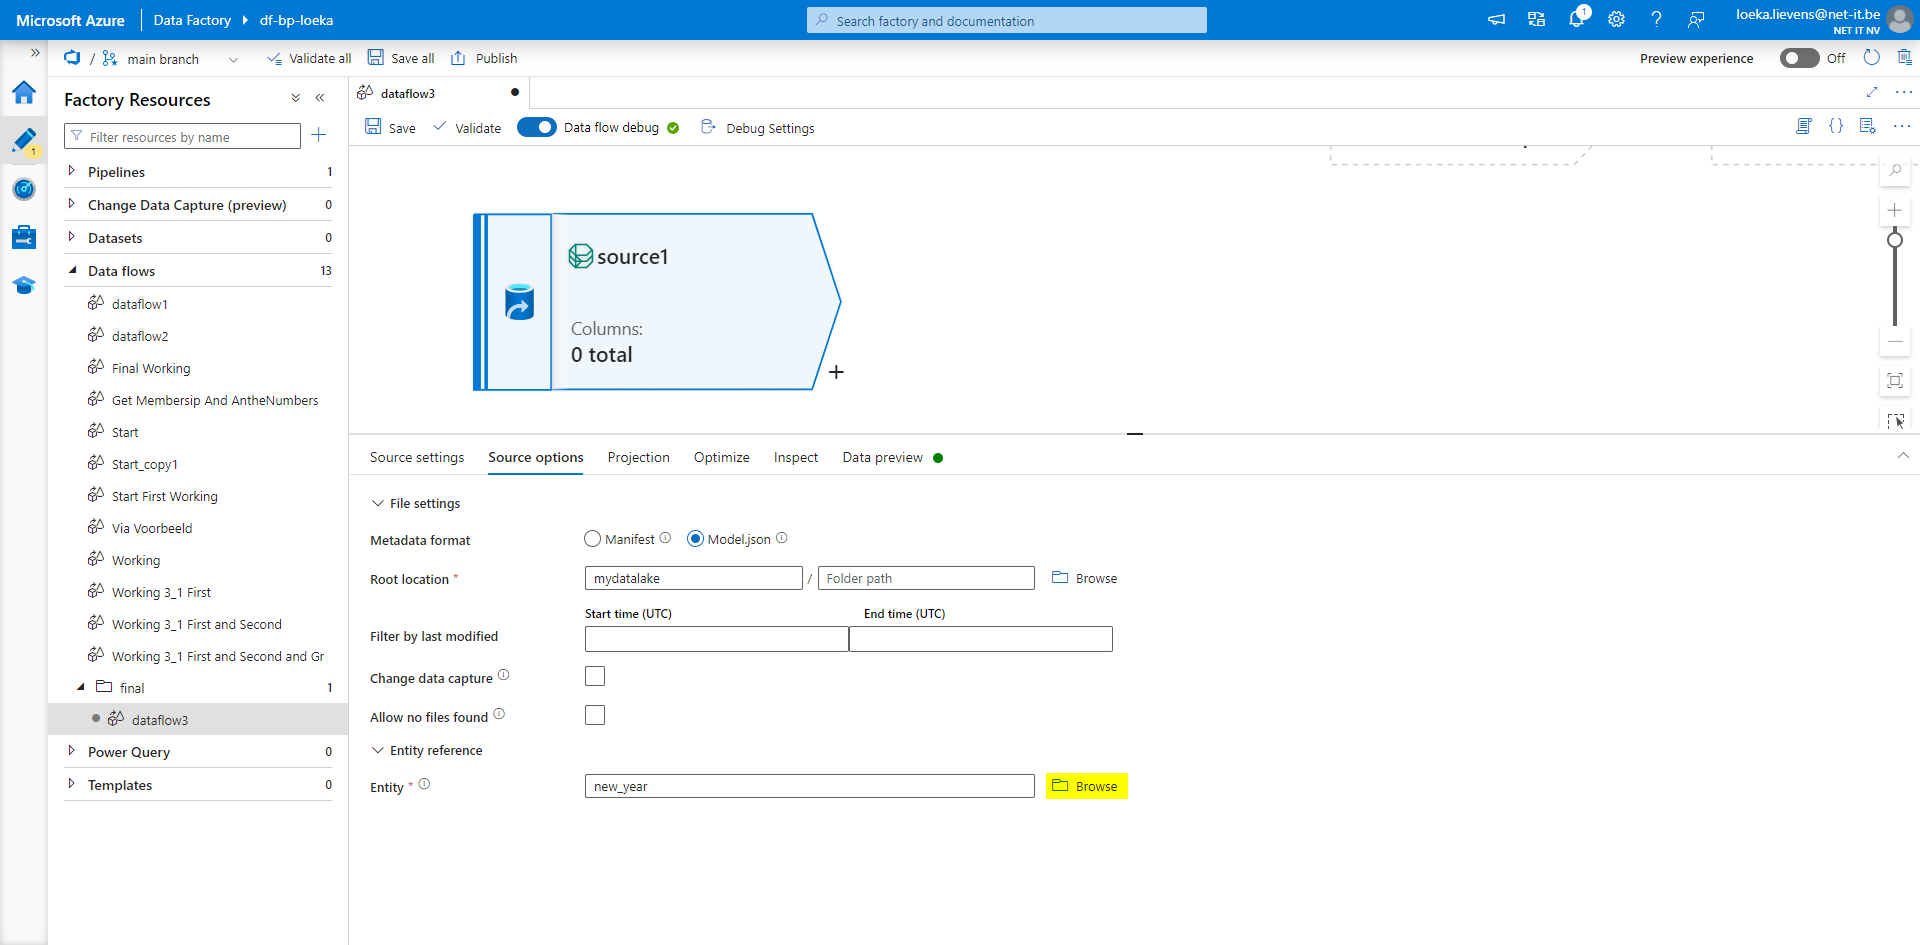
\includegraphics[width=1\textwidth]{./graphics/adf/source_table_5.png}
%\end{center}
%
%Naast `Entity` kunnen we nu op `Browse` klikken om de gewenste entity te gaan importeren. Let op: hier voor zal Data flow debug aan moeten staan.
%
%\begin{center}
%    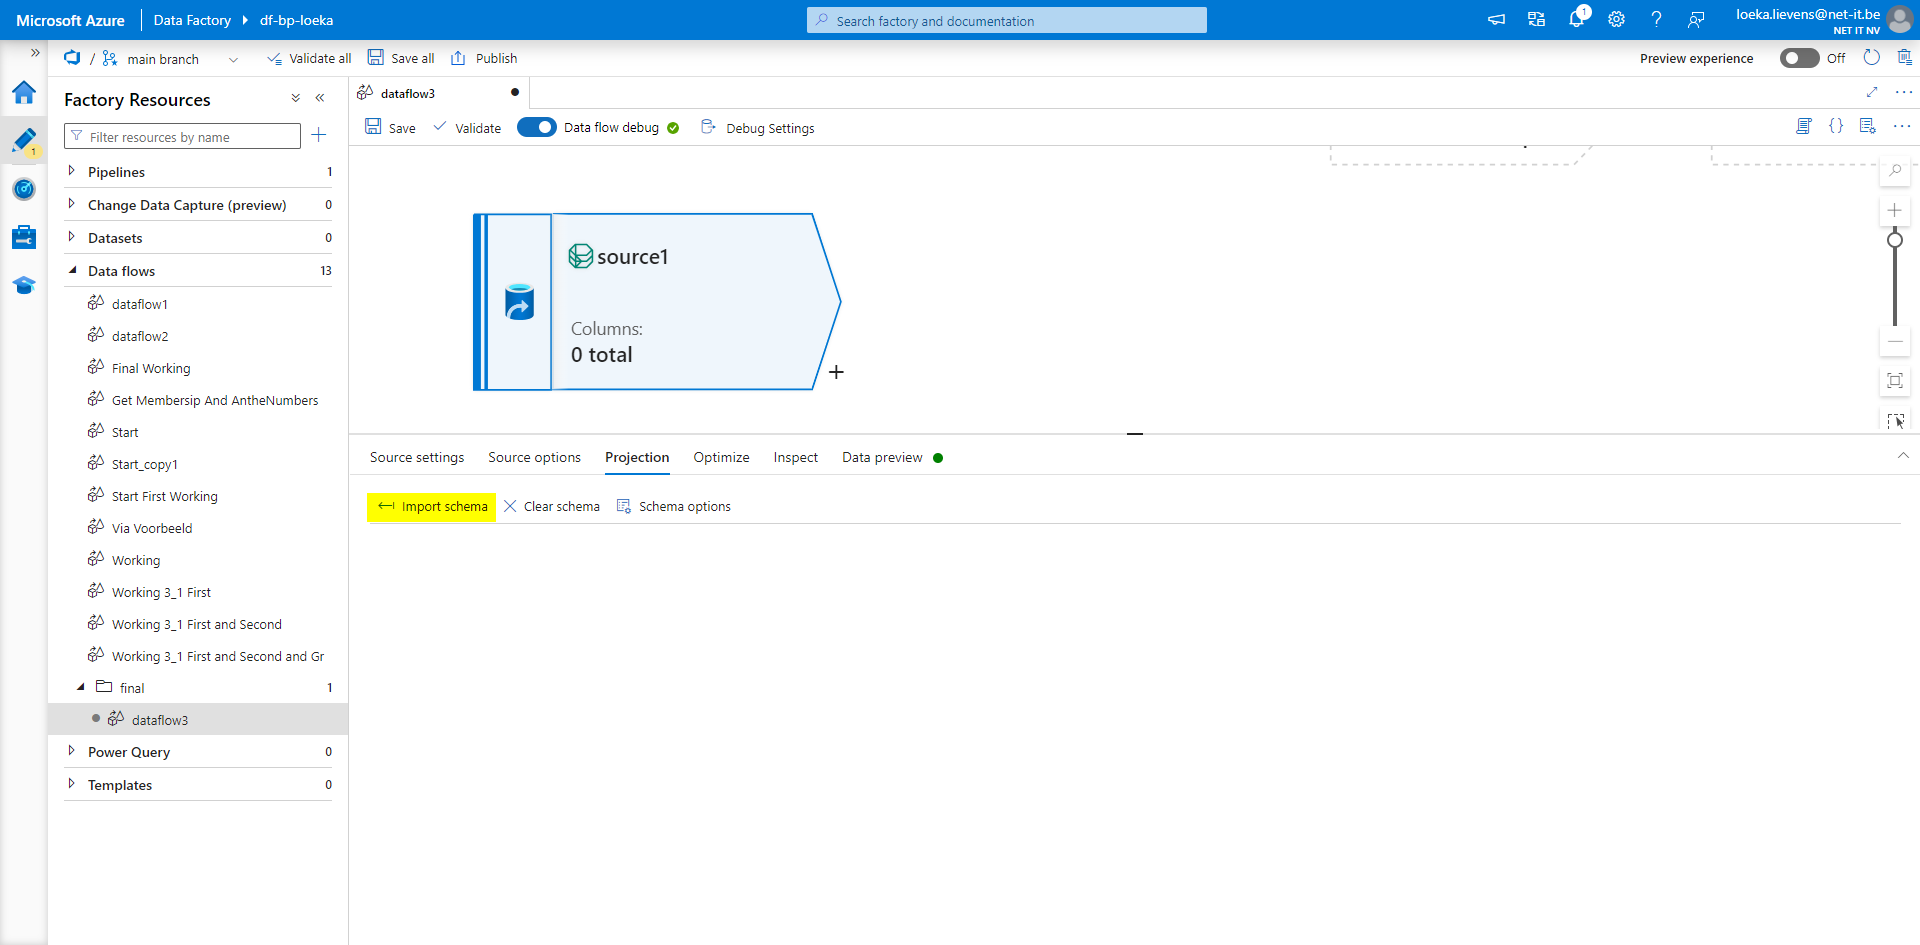
\includegraphics[width=1\textwidth]{./graphics/adf/source_table_6.png}
%\end{center}
%
%Door naar `Projection` te gaan kunnen we nu op `Import schema` klikken.
%
%\begin{center}
%    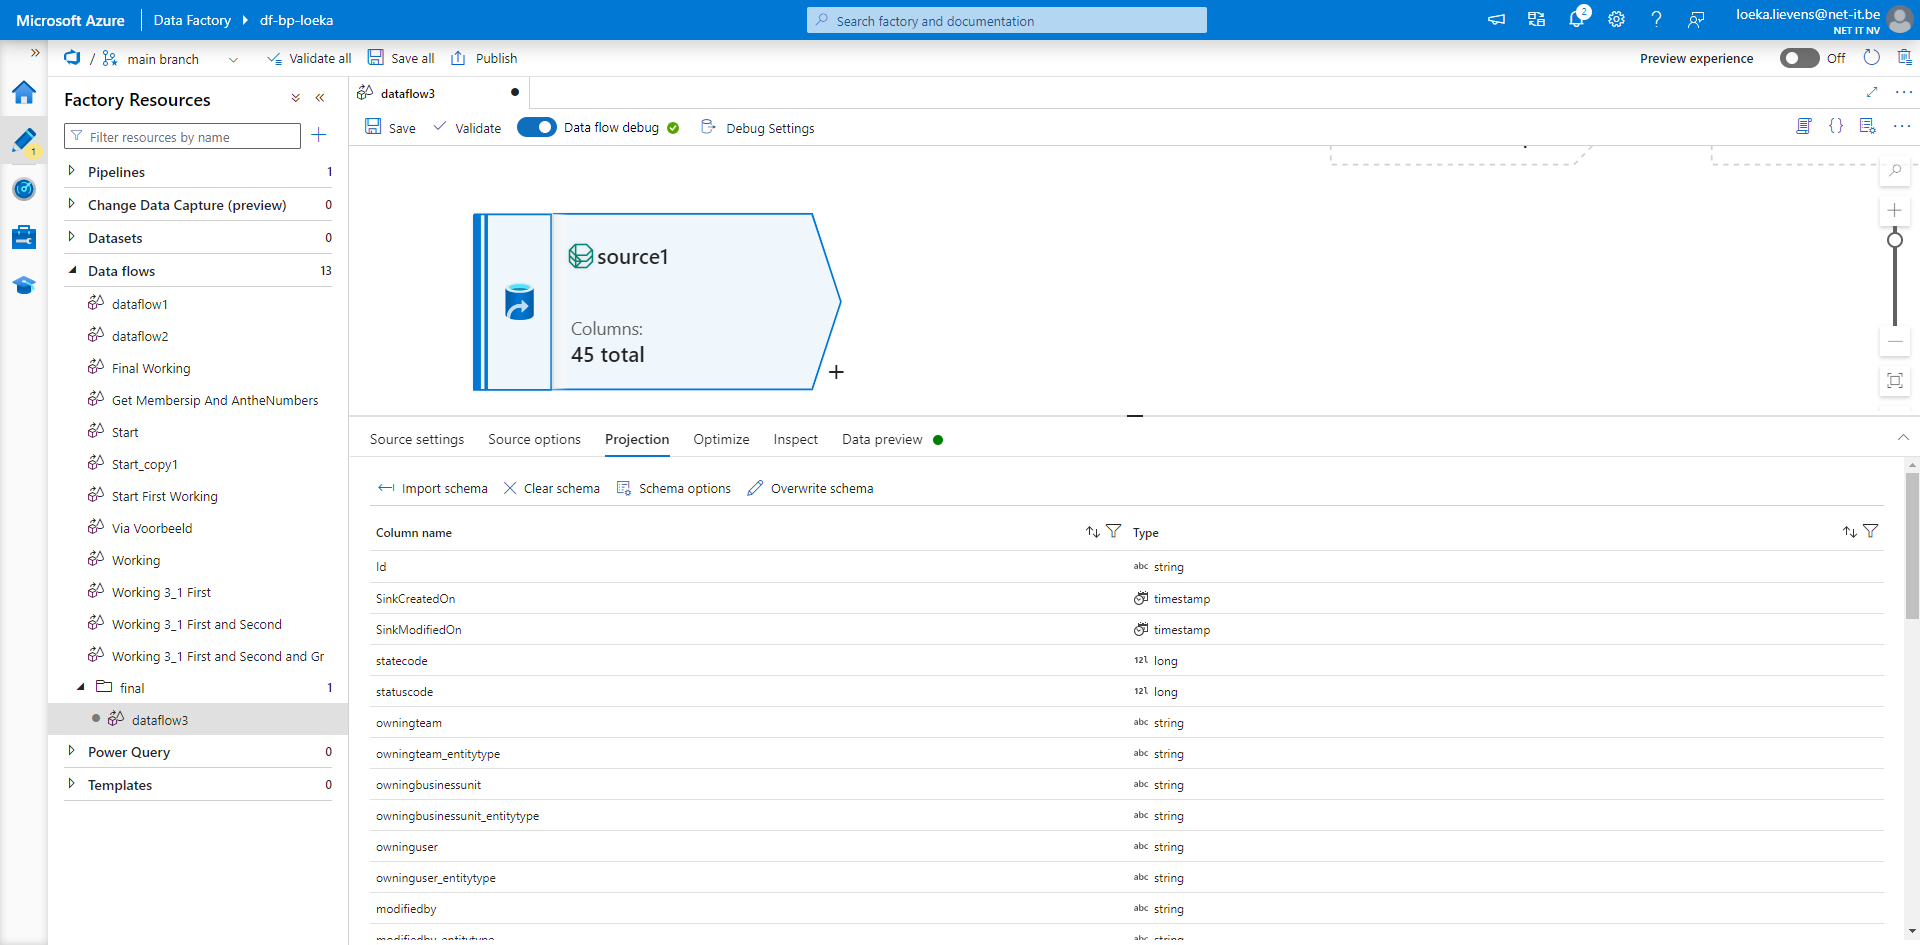
\includegraphics[width=1\textwidth]{./graphics/adf/source_table_7.png}
%\end{center}
%
%De foto hierboven toont een voorbeeld van een geïmporteerd schema.
%
%\begin{center}
%    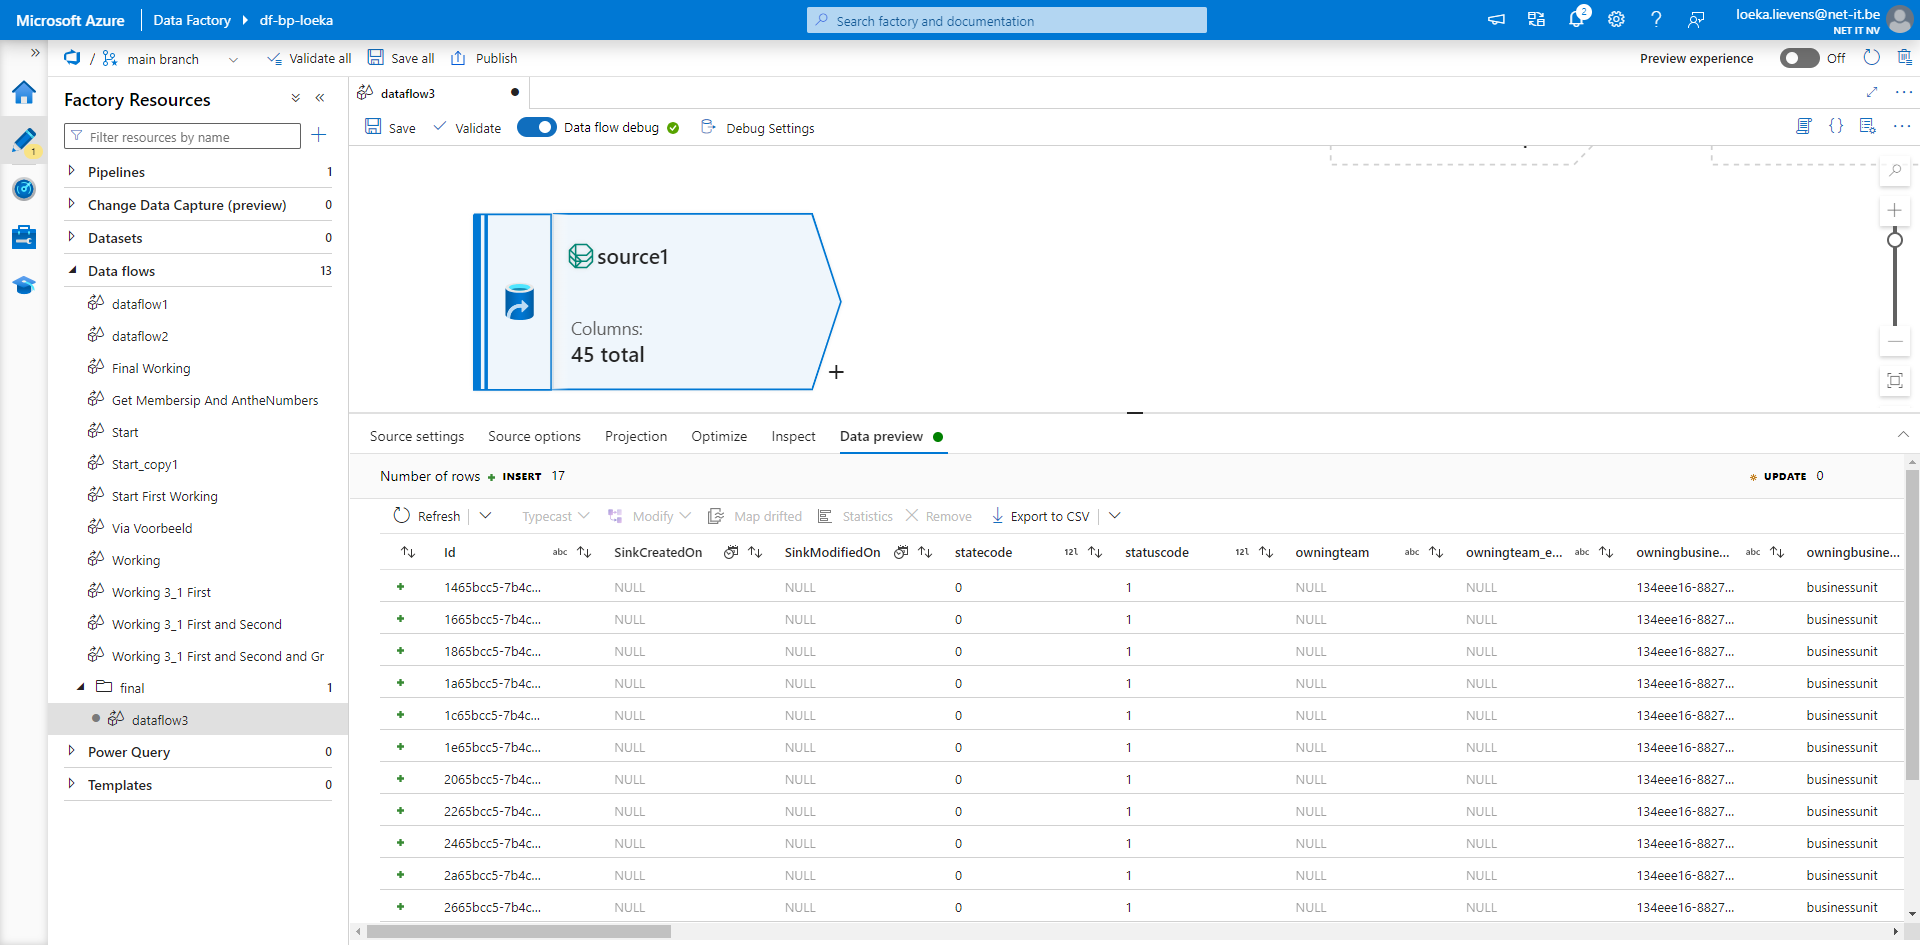
\includegraphics[width=1\textwidth]{./graphics/adf/source_table_8.png}
%\end{center}
%
%Wanneer we naar `Data preview` gaan kunnen we een preview zien van de data uit de gekozen tabel.
%
%\subsubsection{Implementatie ETL}
%
%\begin{center}
%    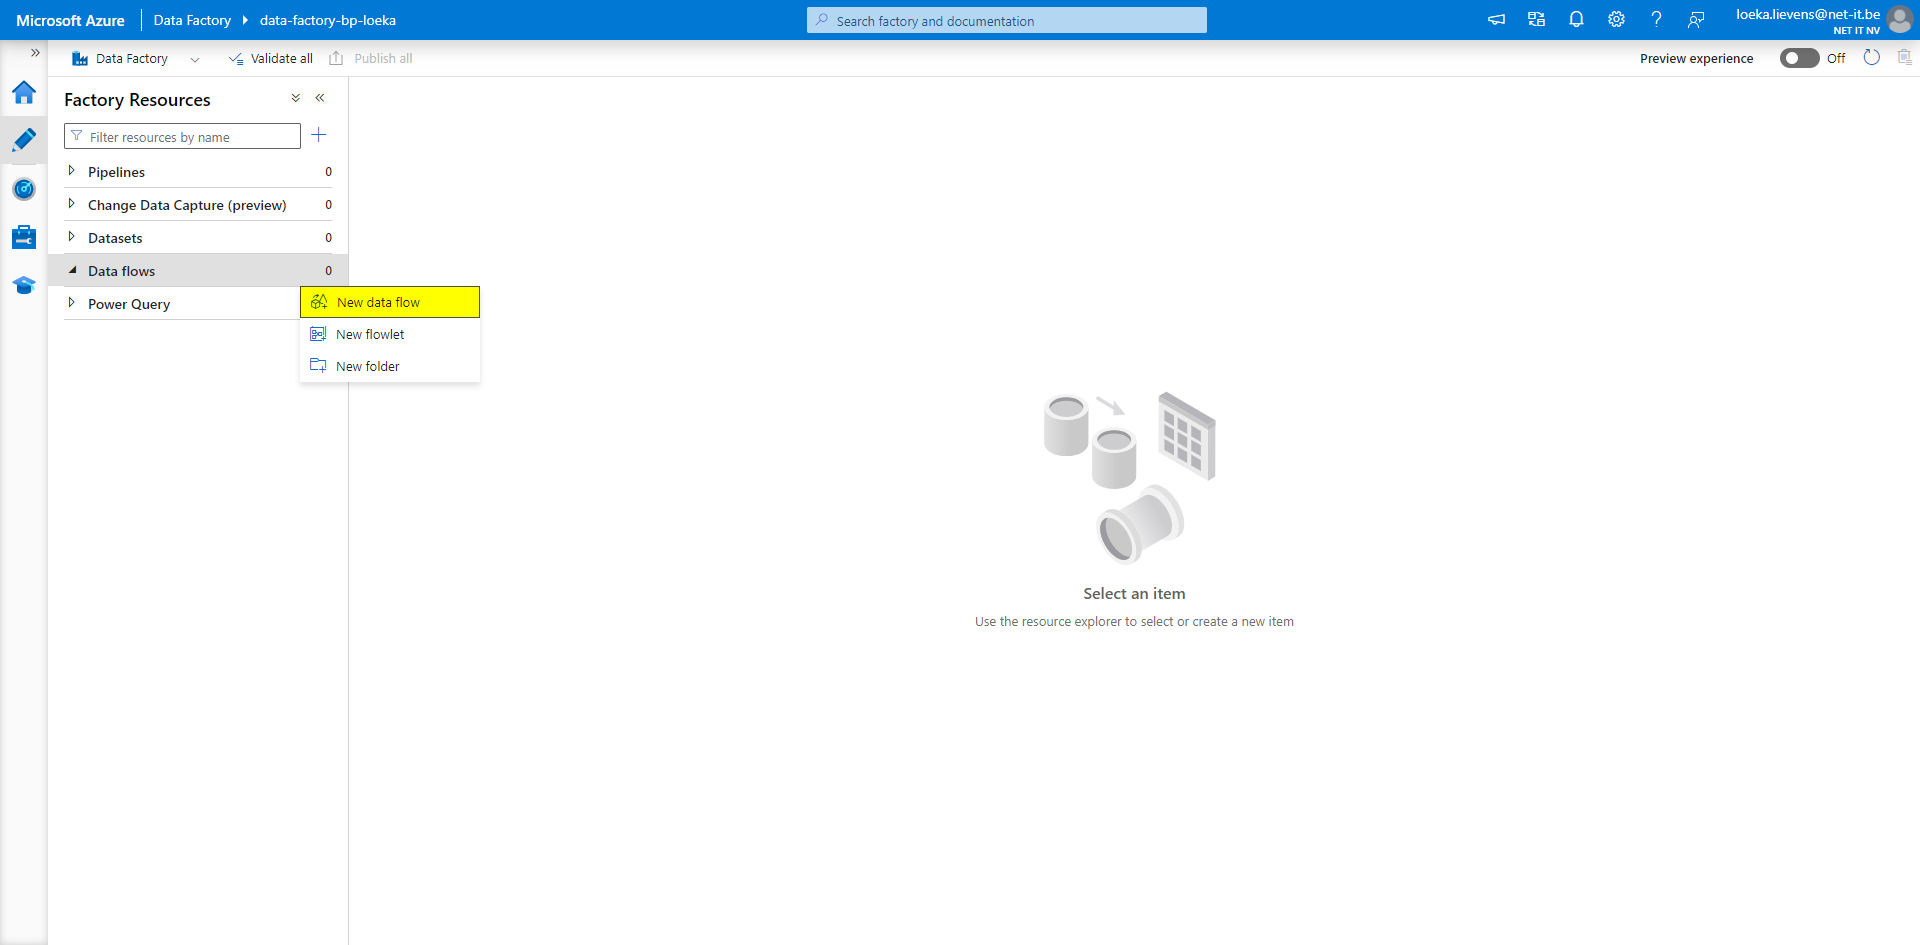
\includegraphics[width=1\textwidth]{./graphics/adf/dataflow.png}
%\end{center}
%
%Voor het implementeren van onze ETL gaan we een nieuwe dataflow gaan aanmaken.
%
%\paragraph{\texttt{Tabel new\_person}}
%
%\begin{center}
%    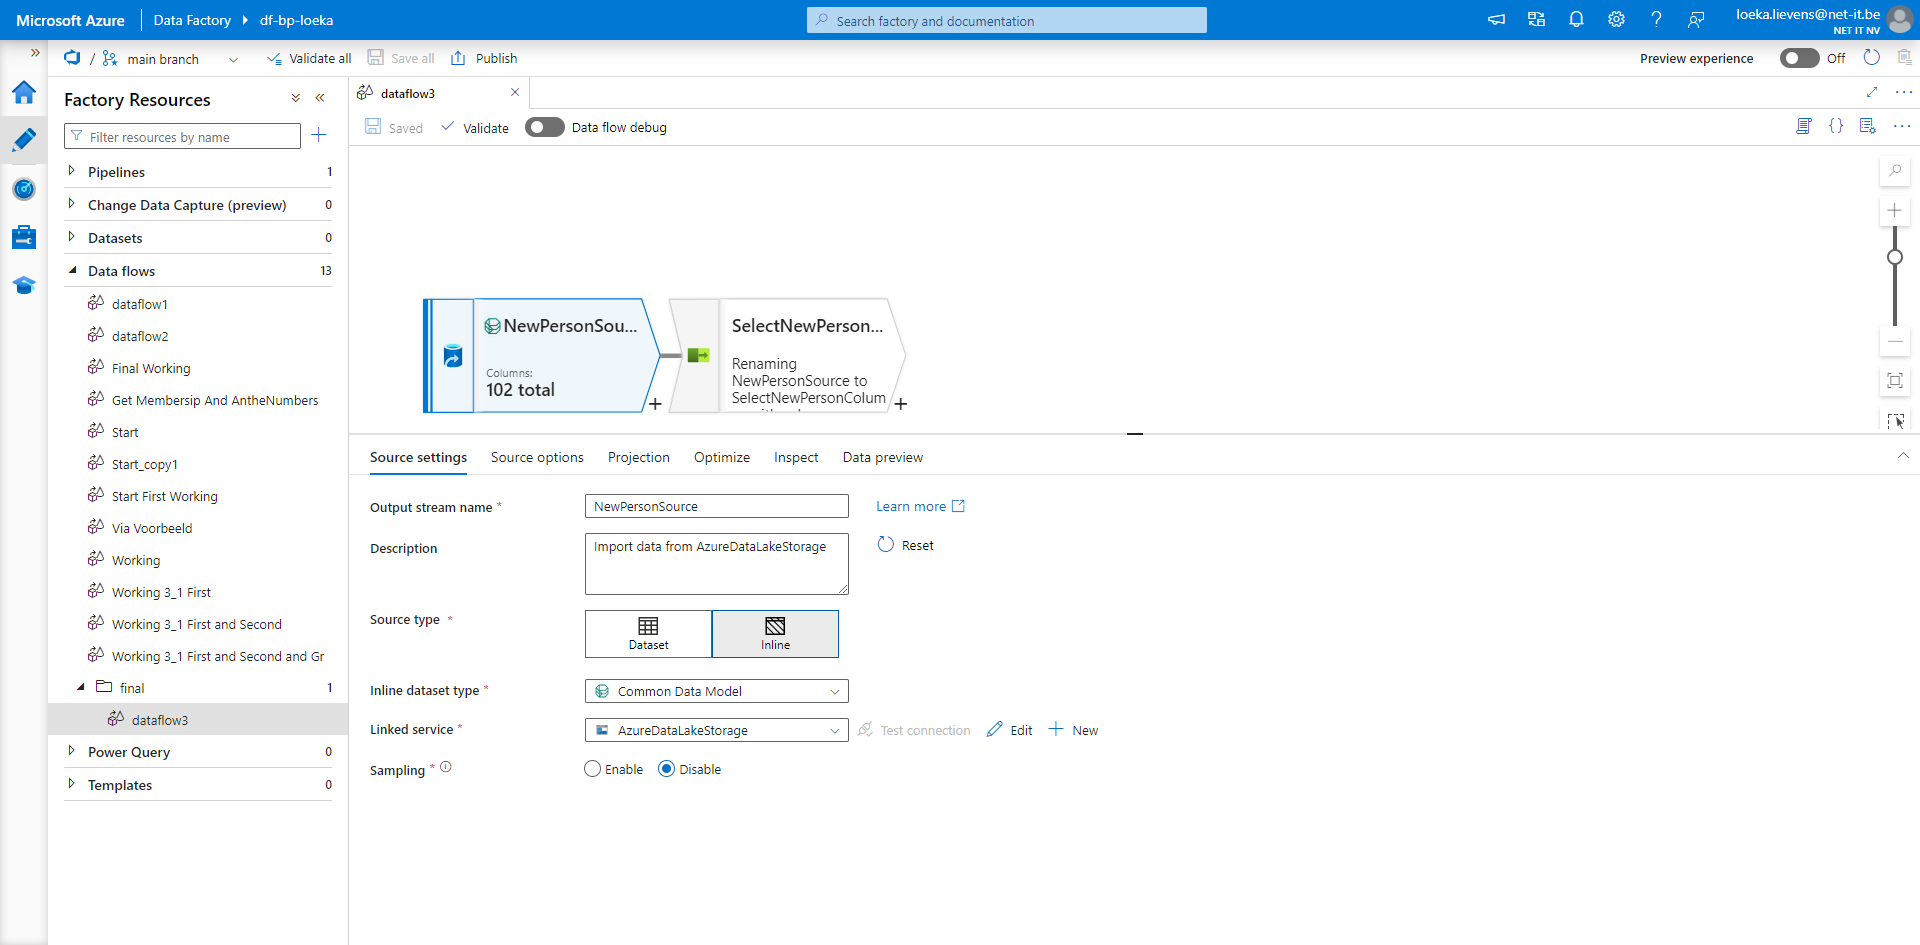
\includegraphics[width=1\textwidth]{./graphics/adf/new_person_source.png}
%\end{center}
%
%\texttt{Er wordt een source toegevoegd voor de tabel new\_person.}
%
%\begin{center}
%    \includegraphics[width=1\textwidth]{./graphics/adf/new_person_select.png}
%\end{center}
%
%\texttt{De nodige kolommen worden geselecteerd en hernoemt met de prefix `p\_`.}
%
%\paragraph{\texttt{Tabel new\_bankaccount}}
%
%\begin{center}
%    \includegraphics[width=1\textwidth]{./graphics/adf/new_bankaccount_source.png}
%\end{center}
%
%\texttt{Er wordt een source toegevoegd voor de tabel new\_bankaccount.}
%
%\begin{center}
%    \includegraphics[width=1\textwidth]{./graphics/adf/new_bankaccount_select.png}
%\end{center}
%
%\texttt{De nodige kolommen worden geselecteerd en hernoemt met de prefix `ba\_`.}
%
%\paragraph{\texttt{Tabel new\_year}}
%
%\begin{center}
%    \includegraphics[width=1\textwidth]{./graphics/adf/new_year_source.png}
%\end{center}
%
%\texttt{Er wordt een source toegevoegd voor de tabel new\_year.}
%
%\begin{center}
%    \includegraphics[width=1\textwidth]{./graphics/adf/new_year_select.png}
%\end{center}
%
%\texttt{De nodige kolommen worden geselecteerd en hernoemt met de prefix `ny\_`.}
%
%\paragraph{\texttt{Tabel new\_group}}
%
%\begin{center}
%    \includegraphics[width=1\textwidth]{./graphics/adf/new_group_source.png}
%\end{center}
%
%\texttt{Er wordt een source toegevoegd voor de tabel new\_group.}
%
%\begin{center}
%    \includegraphics[width=1\textwidth]{./graphics/adf/new_group_select.png}
%\end{center}
%
%\texttt{De nodige kolommen worden geselecteerd en hernoemt met de prefix `ng\_`.}
%
%\paragraph{\texttt{Tabel new\_organizationyear}}
%
%\begin{center}
%    \includegraphics[width=1\textwidth]{./graphics/adf/new_organizationyear_source.png}
%\end{center}
%
%\texttt{Er wordt een source toegevoegd voor de tabel new\_organizationyear.}
%
%\begin{center}
%    \includegraphics[width=1\textwidth]{./graphics/adf/new_organizationyear_select.png}
%\end{center}
%
%\texttt{De nodige kolommen worden geselecteerd en hernoemt met de prefix `noy\_`.}
%
%\begin{center}
%    \includegraphics[width=1\textwidth]{./graphics/adf/new_organizationyear_lookup.png}
%\end{center}
%
%\texttt{De tabel new\_group wordt gejoind met een lookup aan de hand van id.}
%
%% TODO: Link naar juiste foto?
%
%\begin{center}
%    \includegraphics[width=1\textwidth]{./graphics/adf/new_organizationyear_final.png}
%\end{center}
%
%\texttt{We selecteren alle kolommen behalve de kolom met naam ng\_id aangezien deze steeds hetzelfde zal zijn als noy\_new\_groupid.}
%
%\paragraph{\texttt{Tabel new\_membership}}
%
%\begin{center}
%    \includegraphics[width=1\textwidth]{./graphics/adf/new_membership_source.png}
%\end{center}
%
%\texttt{Er wordt een source toegevoegd voor de tabel new\_membership.}
%
%\begin{center}
%    \includegraphics[width=1\textwidth]{./graphics/adf/new_membership_select.png}
%\end{center}
%
%\texttt{De nodige kolommen worden geselecteerd en hernoemt met de prefix `membership\_`.}
%
%\begin{center}
%    \includegraphics[width=1\textwidth]{./graphics/adf/new_membership_filter_1.png}
%\end{center}
%
%\begin{center}
%    \includegraphics[width=1\textwidth]{./graphics/adf/new_membership_filter_2.png}
%\end{center}
%
%\texttt{De membership records worden gefilterd aan de hand van `new\_f30statuscode`, `new\_memberstatuscode` en `new\_aclvbstatuscode`.}
%
%\begin{center}
%    \includegraphics[width=1\textwidth]{./graphics/adf/new_membership_join_1.png}
%\end{center}
%
%\texttt{De tabel new\_group wordt gejoind aan de hand van id.}
%
%\begin{center}
%    \includegraphics[width=1\textwidth]{./graphics/adf/new_membership_join_2.png}
%\end{center}
%
%\texttt{De tabel new\_year wordt gejoind aan de hand van id.}
%
%\begin{center}
%    \includegraphics[width=1\textwidth]{./graphics/adf/new_membership_secondselect_1.png}
%\end{center}
%
%\begin{center}
%    \includegraphics[width=1\textwidth]{./graphics/adf/new_membership_secondselect_2.png}
%\end{center}
%
%\texttt{De kolom `ny\_new\_year` wordt hernoemd naar `membership\_new\_year` en meerdere kolommon worden ongeselecteerd.}
%
%\begin{center}
%    \includegraphics[width=1\textwidth]{./graphics/adf/new_membership_derive.png}
%\end{center}
%
%\texttt{`membership\_new\_year` wordt geparsed naar een integer.}
%
%\begin{center}
%    \includegraphics[width=1\textwidth]{./graphics/adf/new_membership_remove.png}
%\end{center}
%
%\begin{center}
%    \includegraphics[width=1\textwidth]{./graphics/adf/new_membership_remove_2.png}
%\end{center}
%
%Meerdere kolommen worden ongeselecteerd.
%
%\paragraph{\texttt{Tabel new\_syndicalpremiumrequest}}
%
%\begin{center}
%    \includegraphics[width=1\textwidth]{./graphics/adf/spr_source.png}
%\end{center}
%
%\texttt{Er wordt een source toegevoegd voor de tabel new\_syndicalpremiumrequest. Na deze source is er een split, bij het bovenste gaan de kolommen voor de related syndical premium requests geselecteerd worden. Deze zijn belangrijk aangezien dit later gejoind wordt op syndical premium requests.}
%
%\begin{center}
%    \includegraphics[width=1\textwidth]{./graphics/adf/spr_rpr_1.png}
%\end{center}
%
%\begin{center}
%    \includegraphics[width=1\textwidth]{./graphics/adf/spr_rpr_2.png}
%\end{center}
%
%\texttt{De nodige kolommen voor de related syndical premium requests worden geselecteerd en hernoemt met de prefix `rpr\_`.}
%
%\begin{center}
%    \includegraphics[width=1\textwidth]{./graphics/adf/spr_select.png}
%\end{center}
%
%\texttt{De nodige kolommen die gebruikt worden verder in de pipeline worden geselecteerd en hernoemt met de prefix `spr\_`. Ook zijn er kolommen zonder deze prefix, deze zullen later in het export bestand terecht komen.}
%
%\begin{center}
%    \includegraphics[width=1\textwidth]{./graphics/adf/spr_join_person.png}
%\end{center}
%
%\texttt{De tabel new\_person wordt gejoind aan de hand van id.}
%
%\begin{center}
%    \includegraphics[width=1\textwidth]{./graphics/adf/spr_join_bankaccount.png}
%\end{center}
%
%\texttt{De tabel new\_bankaccount wordt gejoind aan de hand van id.}
%
%\begin{center}
%    \includegraphics[width=1\textwidth]{./graphics/adf/spr_join_rpr.png}
%\end{center}
%
%\texttt{De related premium requests worden gejoind aan de hand van id.}
%
%\begin{center}
%    \includegraphics[width=1\textwidth]{./graphics/adf/spr_join_year.png}
%\end{center}
%
%\texttt{De tabel new\_year wordt gejoind aan de hand van id.}
%
%\begin{center}
%    \includegraphics[width=1\textwidth]{./graphics/adf/spr_derive_1.png}
%\end{center}
%
%Er worden kolommen berekend die later in het export bestand zullen terecht komen.
%
%\begin{center}
%    \includegraphics[width=1\textwidth]{./graphics/adf/spr_derive_2.png}
%\end{center}
%
%\texttt{De kolommen `EntryYear`, `CalendarYear` en `RefYear` zijn belangrijk. Met behulp van deze kolommen wordt er gekeken naar welke groepen een bepaalde premie (new\_syndicalpremiumrequest) zal gestuurd moeten worden.}
%
%\begin{center}
%    \includegraphics[width=1\textwidth]{./graphics/adf/spr_rename_1.png}
%\end{center}
%
%\begin{center}
%    \includegraphics[width=1\textwidth]{./graphics/adf/spr_rename_2.png}
%\end{center}
%
%Ook nu worden er kolommen hernoemd die in het export bestand zullen terecht komen. Daarnaast zijn er ook kolommen die ongeselecteerd worden doordat we deze verder in de pipeline niet meer nodig hebben.